\documentclass[a4paper]{book}
\usepackage{a4wide}
\usepackage{makeidx}
\usepackage{fancyhdr}
\usepackage{graphicx}
\usepackage{multicol}
\usepackage{float}
\usepackage{textcomp}
\usepackage{alltt}
\usepackage{times}
\usepackage{ifpdf}
\ifpdf
\usepackage[pdftex,
            pagebackref=true,
            colorlinks=true,
            linkcolor=blue
           ]{hyperref}
\else
\usepackage[ps2pdf,
            pagebackref=true,
            colorlinks=true,
            linkcolor=blue
           ]{hyperref}
\usepackage{pspicture}
\fi
\usepackage{doxygen}
\usepackage{hyperref}
\makeindex
\setcounter{tocdepth}{1}
\renewcommand{\footrulewidth}{0.4pt}
\begin{document}
\begin{titlepage}
\vspace*{7cm}
\begin{center}
{\Large coin Reference Manual}\\
\vspace*{1cm}
{\large Generated by Doxygen 1.4.6}\\
\vspace*{0.5cm}
{\small Tue Apr 24 16:56:50 2007}\\
\end{center}
\end{titlepage}
\clearemptydoublepage
\pagenumbering{roman}
\tableofcontents
\clearemptydoublepage
\pagenumbering{arabic}
\chapter{coin Directory Hierarchy}
\section{Directories}
This directory hierarchy is sorted roughly, but not completely, alphabetically:\begin{DoxyCompactList}
\item \contentsline{section}{src}{\pageref{dir_490b8ab9500c911a5be23e756ab981a7}}{}
\end{DoxyCompactList}

\chapter{coin Hierarchical Index}
\section{coin Class Hierarchy}
This inheritance list is sorted roughly, but not completely, alphabetically:\begin{CompactList}
\item \contentsline{section}{cel\-W}{\pageref{structcelW}}{}
\end{CompactList}

\chapter{coin Class Index}
\section{Class List}
Here are the classes, structs, unions and interfaces with brief descriptions:\begin{CompactList}
\item\contentsline{section}{\hyperlink{structcelW}{celW} }{\pageref{structcelW}}{}
\end{CompactList}

\chapter{coin File Index}
\section{File List}
Here is a list of all files with brief descriptions:\begin{CompactList}
\item\contentsline{section}{\hyperlink{Classes_8c}{Classes.c} }{\pageref{Classes_8c}}{}
\item\contentsline{section}{\hyperlink{Classes_8h}{Classes.h} }{\pageref{Classes_8h}}{}
\item\contentsline{section}{\hyperlink{coin__common_8h}{coin\_\-common.h} }{\pageref{coin__common_8h}}{}
\item\contentsline{section}{\hyperlink{Helpers_8c}{Helpers.c} }{\pageref{Helpers_8c}}{}
\item\contentsline{section}{\hyperlink{Helpers_8h}{Helpers.h} }{\pageref{Helpers_8h}}{}
\item\contentsline{section}{\hyperlink{LinearStatistic_8c}{LinearStatistic.c} }{\pageref{LinearStatistic_8c}}{}
\item\contentsline{section}{\hyperlink{LinearStatistic_8h}{LinearStatistic.h} }{\pageref{LinearStatistic_8h}}{}
\item\contentsline{section}{\hyperlink{StreitbergRoehmel_8c}{StreitbergRoehmel.c} }{\pageref{StreitbergRoehmel_8c}}{}
\item\contentsline{section}{\hyperlink{vandeWiel_8c}{vandeWiel.c} }{\pageref{vandeWiel_8c}}{}
\end{CompactList}

\chapter{coin Directory Documentation}
\hypertarget{dir_ffcd7fcaa547dc02c1b00308358d1322}{
\section{src/ Directory Reference}
\label{dir_ffcd7fcaa547dc02c1b00308358d1322}\index{src/ Directory Reference@{src/ Directory Reference}}
}


\begin{figure}[H]
\begin{center}
\leavevmode
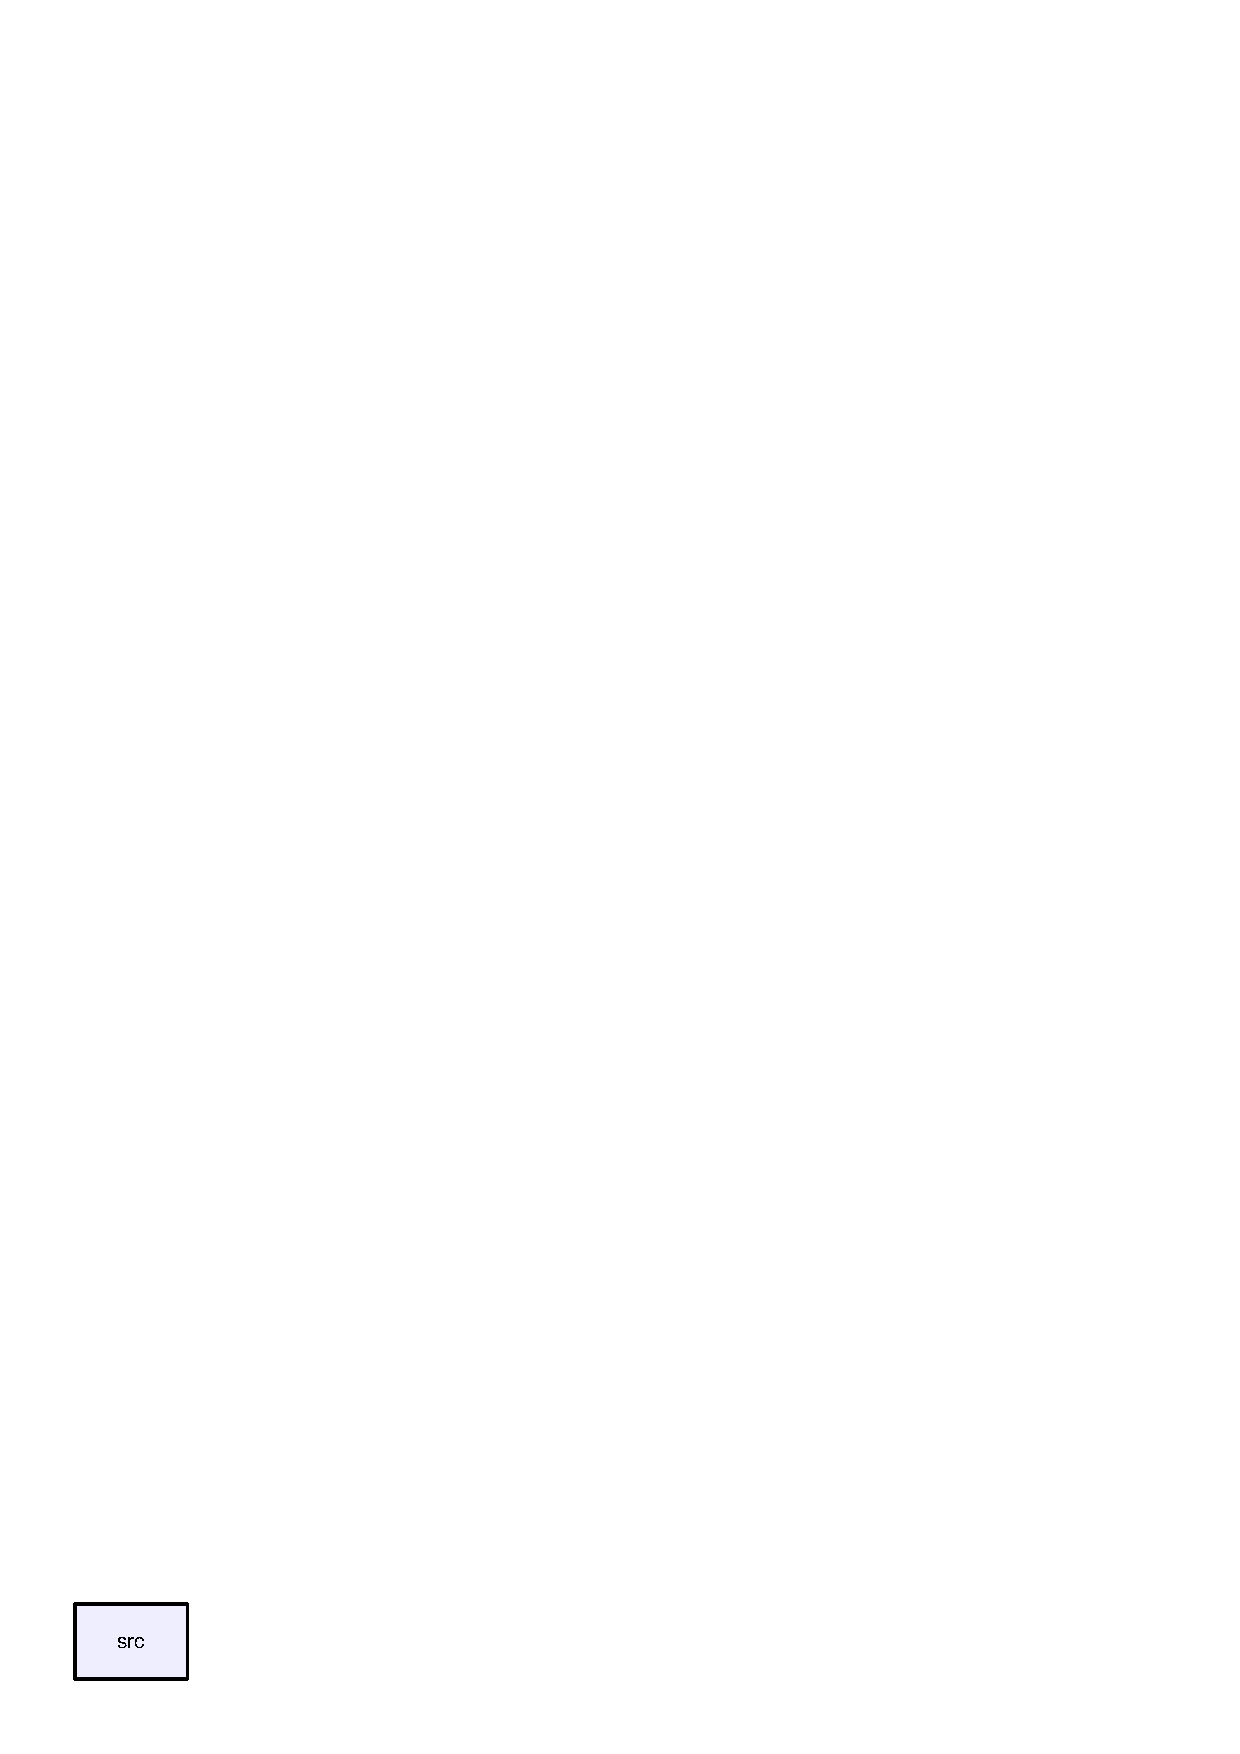
\includegraphics[width=45pt]{dir_ffcd7fcaa547dc02c1b00308358d1322_dep}
\end{center}
\end{figure}
\subsection*{Files}
\begin{CompactItemize}
\item 
file \hyperlink{Classes_8c}{Classes.c}
\item 
file \hyperlink{Classes_8h}{Classes.h}
\item 
file \hyperlink{coin__common_8h}{coin\_\-common.h}
\item 
file \hyperlink{Helpers_8c}{Helpers.c}
\item 
file \hyperlink{Helpers_8h}{Helpers.h}
\item 
file \hyperlink{LinearStatistic_8c}{Linear\-Statistic.c}
\item 
file \hyperlink{LinearStatistic_8h}{Linear\-Statistic.h}
\item 
file \hyperlink{StreitbergRoehmel_8c}{Streitberg\-Roehmel.c}
\item 
file \hyperlink{vandeWiel_8c}{vande\-Wiel.c}
\end{CompactItemize}

\chapter{coin Class Documentation}
\hypertarget{structcelW}{
\section{celW Struct Reference}
\label{structcelW}\index{celW@{celW}}
}
\subsection*{Public Attributes}
\begin{CompactItemize}
\item 
long \hyperlink{structcelW_47b173a5f8c56a051237cac49ddbef4f}{length}
\item 
double $\ast$ \hyperlink{structcelW_f8a631c01b9310cf542171f4df975499}{c}
\item 
double $\ast$ \hyperlink{structcelW_b443b2a7120f170c2c5e8012f4dd86d7}{x}
\end{CompactItemize}


\subsection{Detailed Description}
The probability distribution for the independent two sample problem.

REFERENCE

M.A. van de Wiel (2001). The split-up algorithm: a fast symbolic method for computing p-values of rank statistics, Computational Statistics, 16, 519-538. 

Definition at line 31 of file vandeWiel.c.

\subsection{Member Data Documentation}
\hypertarget{structcelW_f8a631c01b9310cf542171f4df975499}{
\index{celW@{celW}!c@{c}}
\index{c@{c}!celW@{celW}}
\subsubsection[{c}]{\setlength{\rightskip}{0pt plus 5cm}double$\ast$ {\bf celW::c}}}
\label{structcelW_f8a631c01b9310cf542171f4df975499}




Definition at line 33 of file vandeWiel.c.

Referenced by cumulcoef(), fillcell(), initW(), mirrorW(), mymergesort(), numbersmall(), plus(), and reserveW().\hypertarget{structcelW_47b173a5f8c56a051237cac49ddbef4f}{
\index{celW@{celW}!length@{length}}
\index{length@{length}!celW@{celW}}
\subsubsection[{length}]{\setlength{\rightskip}{0pt plus 5cm}long {\bf celW::length}}}
\label{structcelW_47b173a5f8c56a051237cac49ddbef4f}




Definition at line 32 of file vandeWiel.c.

Referenced by cumulcoef(), fillcell(), initW(), mirrorW(), mult(), mymergesort(), numbersmall(), and plus().\hypertarget{structcelW_b443b2a7120f170c2c5e8012f4dd86d7}{
\index{celW@{celW}!x@{x}}
\index{x@{x}!celW@{celW}}
\subsubsection[{x}]{\setlength{\rightskip}{0pt plus 5cm}double$\ast$ {\bf celW::x}}}
\label{structcelW_b443b2a7120f170c2c5e8012f4dd86d7}




Definition at line 34 of file vandeWiel.c.

Referenced by fillcell(), initW(), mirrorW(), mymergesort(), plus(), and reserveW().

The documentation for this struct was generated from the following file:\begin{CompactItemize}
\item 
\hyperlink{vandeWiel_8c}{vandeWiel.c}\end{CompactItemize}

\chapter{coin File Documentation}
\hypertarget{Classes_8c}{
\section{Classes.c File Reference}
\label{Classes_8c}\index{Classes.c@{Classes.c}}
}
{\ttfamily \#include \char`\"{}coin\_\-common.h\char`\"{}}\par
Include dependency graph for Classes.c:
\nopagebreak
\begin{figure}[H]
\begin{center}
\leavevmode
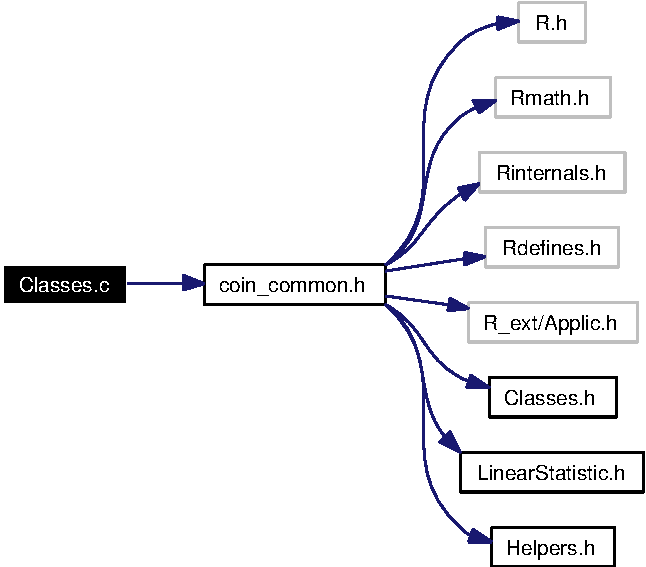
\includegraphics[width=400pt]{Classes_8c__incl}
\end{center}
\end{figure}
\subsection*{Functions}
\begin{DoxyCompactItemize}
\item 
SEXP \hyperlink{Classes_8c_a5d60a29bf291202b78048a4cd7265a32}{coin\_\-init} (void)
\end{DoxyCompactItemize}
\subsection*{Variables}
\begin{DoxyCompactItemize}
\item 
SEXP \hyperlink{Classes_8c_abbb9eebf67e5de25bd14a119d80547c8}{coin\_\-expectationSym}
\item 
SEXP \hyperlink{Classes_8c_af9d3f842579c178af113bdaae30eda44}{coin\_\-covarianceSym}
\item 
SEXP \hyperlink{Classes_8c_aacb7ca69262bcec0b61014b0a152672b}{coin\_\-sumweightsSym}
\end{DoxyCompactItemize}


\subsection{Detailed Description}
S4 classes

\begin{DoxyAuthor}{Author}

\end{DoxyAuthor}
\begin{DoxyParagraph}{Author:}
hothorn 
\end{DoxyParagraph}
\begin{DoxyDate}{Date}

\end{DoxyDate}
\begin{DoxyParagraph}{Date:}
2007-\/02-\/15 09:25:46 +0100 (Thu, 15 Feb 2007) 
\end{DoxyParagraph}


Definition in file \hyperlink{Classes_8c_source}{Classes.c}.



\subsection{Function Documentation}
\hypertarget{Classes_8c_a5d60a29bf291202b78048a4cd7265a32}{
\index{Classes.c@{Classes.c}!coin\_\-init@{coin\_\-init}}
\index{coin\_\-init@{coin\_\-init}!Classes.c@{Classes.c}}
\subsubsection[{coin\_\-init}]{\setlength{\rightskip}{0pt plus 5cm}SEXP coin\_\-init (
\begin{DoxyParamCaption}
\item[{void}]{}
\end{DoxyParamCaption}
)}}
\label{Classes_8c_a5d60a29bf291202b78048a4cd7265a32}


Definition at line 16 of file Classes.c.



References coin\_\-covarianceSym, coin\_\-expectationSym, and coin\_\-sumweightsSym.



\subsection{Variable Documentation}
\hypertarget{Classes_8c_af9d3f842579c178af113bdaae30eda44}{
\index{Classes.c@{Classes.c}!coin\_\-covarianceSym@{coin\_\-covarianceSym}}
\index{coin\_\-covarianceSym@{coin\_\-covarianceSym}!Classes.c@{Classes.c}}
\subsubsection[{coin\_\-covarianceSym}]{\setlength{\rightskip}{0pt plus 5cm}SEXP {\bf coin\_\-covarianceSym}}}
\label{Classes_8c_af9d3f842579c178af113bdaae30eda44}


Definition at line 12 of file Classes.c.



Referenced by C\_\-ExpectCovarInfluence(), C\_\-ExpectCovarLinearStatistic(), coin\_\-init(), R\_\-ExpectCovarInfluence(), and R\_\-ExpectCovarLinearStatistic().

\hypertarget{Classes_8c_abbb9eebf67e5de25bd14a119d80547c8}{
\index{Classes.c@{Classes.c}!coin\_\-expectationSym@{coin\_\-expectationSym}}
\index{coin\_\-expectationSym@{coin\_\-expectationSym}!Classes.c@{Classes.c}}
\subsubsection[{coin\_\-expectationSym}]{\setlength{\rightskip}{0pt plus 5cm}SEXP {\bf coin\_\-expectationSym}}}
\label{Classes_8c_abbb9eebf67e5de25bd14a119d80547c8}


Definition at line 12 of file Classes.c.



Referenced by C\_\-ExpectCovarInfluence(), C\_\-ExpectCovarLinearStatistic(), coin\_\-init(), R\_\-ExpectCovarInfluence(), and R\_\-ExpectCovarLinearStatistic().

\hypertarget{Classes_8c_aacb7ca69262bcec0b61014b0a152672b}{
\index{Classes.c@{Classes.c}!coin\_\-sumweightsSym@{coin\_\-sumweightsSym}}
\index{coin\_\-sumweightsSym@{coin\_\-sumweightsSym}!Classes.c@{Classes.c}}
\subsubsection[{coin\_\-sumweightsSym}]{\setlength{\rightskip}{0pt plus 5cm}SEXP {\bf coin\_\-sumweightsSym}}}
\label{Classes_8c_aacb7ca69262bcec0b61014b0a152672b}


Definition at line 12 of file Classes.c.



Referenced by C\_\-ExpectCovarInfluence(), C\_\-ExpectCovarLinearStatistic(), coin\_\-init(), and R\_\-ExpectCovarInfluence().


\hypertarget{Classes_8h}{
\section{Classes.h File Reference}
\label{Classes_8h}\index{Classes.h@{Classes.h}}
}
This graph shows which files directly or indirectly include this file:\nopagebreak
\begin{figure}[H]
\begin{center}
\leavevmode
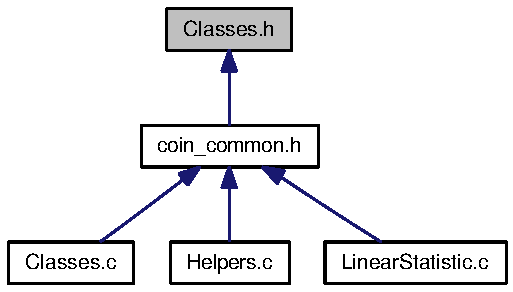
\includegraphics[width=141pt]{Classes_8h__dep__incl}
\end{center}
\end{figure}
\subsection*{Variables}
\begin{DoxyCompactItemize}
\item 
SEXP \hyperlink{Classes_8h_abbb9eebf67e5de25bd14a119d80547c8}{coin\_\-expectationSym}
\item 
SEXP \hyperlink{Classes_8h_af9d3f842579c178af113bdaae30eda44}{coin\_\-covarianceSym}
\item 
SEXP \hyperlink{Classes_8h_aacb7ca69262bcec0b61014b0a152672b}{coin\_\-sumweightsSym}
\end{DoxyCompactItemize}


\subsection{Variable Documentation}
\hypertarget{Classes_8h_af9d3f842579c178af113bdaae30eda44}{
\index{Classes.h@{Classes.h}!coin\_\-covarianceSym@{coin\_\-covarianceSym}}
\index{coin\_\-covarianceSym@{coin\_\-covarianceSym}!Classes.h@{Classes.h}}
\subsubsection[{coin\_\-covarianceSym}]{\setlength{\rightskip}{0pt plus 5cm}SEXP {\bf coin\_\-covarianceSym}}}
\label{Classes_8h_af9d3f842579c178af113bdaae30eda44}


Definition at line 12 of file Classes.c.

Referenced by C\_\-ExpectCovarInfluence(), C\_\-ExpectCovarLinearStatistic(), coin\_\-init(), R\_\-ExpectCovarInfluence(), and R\_\-ExpectCovarLinearStatistic().\hypertarget{Classes_8h_abbb9eebf67e5de25bd14a119d80547c8}{
\index{Classes.h@{Classes.h}!coin\_\-expectationSym@{coin\_\-expectationSym}}
\index{coin\_\-expectationSym@{coin\_\-expectationSym}!Classes.h@{Classes.h}}
\subsubsection[{coin\_\-expectationSym}]{\setlength{\rightskip}{0pt plus 5cm}SEXP {\bf coin\_\-expectationSym}}}
\label{Classes_8h_abbb9eebf67e5de25bd14a119d80547c8}


Definition at line 12 of file Classes.c.

Referenced by C\_\-ExpectCovarInfluence(), C\_\-ExpectCovarLinearStatistic(), coin\_\-init(), R\_\-ExpectCovarInfluence(), and R\_\-ExpectCovarLinearStatistic().\hypertarget{Classes_8h_aacb7ca69262bcec0b61014b0a152672b}{
\index{Classes.h@{Classes.h}!coin\_\-sumweightsSym@{coin\_\-sumweightsSym}}
\index{coin\_\-sumweightsSym@{coin\_\-sumweightsSym}!Classes.h@{Classes.h}}
\subsubsection[{coin\_\-sumweightsSym}]{\setlength{\rightskip}{0pt plus 5cm}SEXP {\bf coin\_\-sumweightsSym}}}
\label{Classes_8h_aacb7ca69262bcec0b61014b0a152672b}


Definition at line 12 of file Classes.c.

Referenced by C\_\-ExpectCovarInfluence(), C\_\-ExpectCovarLinearStatistic(), coin\_\-init(), and R\_\-ExpectCovarInfluence().
\hypertarget{coin__common_8h}{
\section{coin\_\-common.h File Reference}
\label{coin__common_8h}\index{coin_common.h@{coin\_\-common.h}}
}
{\tt \#include $<$R.h$>$}\par
{\tt \#include $<$Rmath.h$>$}\par
{\tt \#include $<$Rinternals.h$>$}\par
{\tt \#include $<$Rdefines.h$>$}\par
{\tt \#include $<$R\_\-ext/Applic.h$>$}\par
{\tt \#include \char`\"{}Classes.h\char`\"{}}\par
{\tt \#include \char`\"{}Linear\-Statistic.h\char`\"{}}\par
{\tt \#include \char`\"{}Helpers.h\char`\"{}}\par


Include dependency graph for coin\_\-common.h:\begin{figure}[H]
\begin{center}
\leavevmode
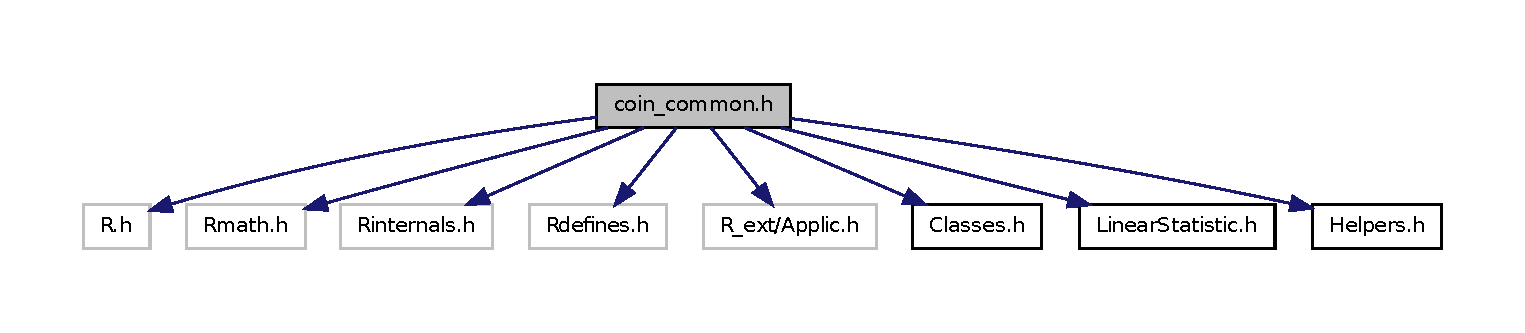
\includegraphics[width=124pt]{coin__common_8h__incl}
\end{center}
\end{figure}


This graph shows which files directly or indirectly include this file:\begin{figure}[H]
\begin{center}
\leavevmode
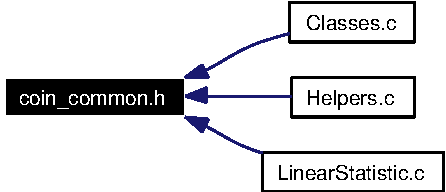
\includegraphics[width=124pt]{coin__common_8h__dep__incl}
\end{center}
\end{figure}

\hypertarget{Helpers_8c}{
\section{Helpers.c File Reference}
\label{Helpers_8c}\index{Helpers.c@{Helpers.c}}
}
{\tt \#include \char`\"{}coin\_\-common.h\char`\"{}}\par


Include dependency graph for Helpers.c:\nopagebreak
\begin{figure}[H]
\begin{center}
\leavevmode
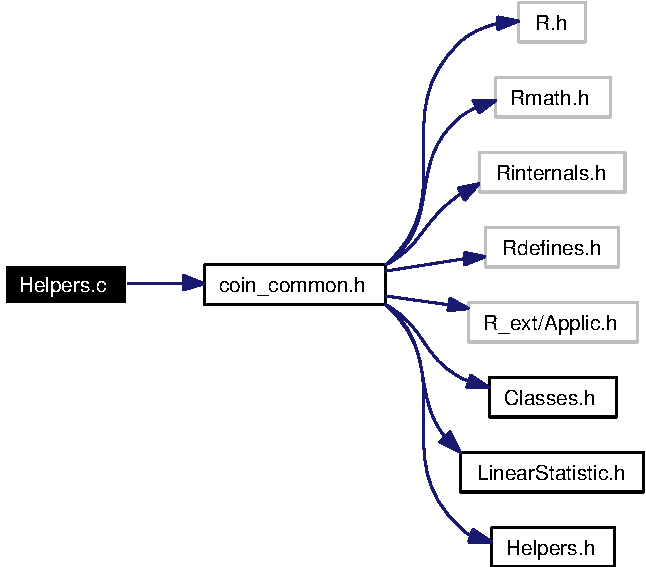
\includegraphics[width=332pt]{Helpers_8c__incl}
\end{center}
\end{figure}
\subsection*{Functions}
\begin{CompactItemize}
\item 
int \hyperlink{Helpers_8c_eeb672a71c45ead28b7b354414f2427a}{nrow} (SEXP x)
\item 
int \hyperlink{Helpers_8c_f1f46cc3e98630497a1ccb21d943fe65}{ncol} (SEXP x)
\item 
void \hyperlink{Helpers_8c_f7c710920d1496d23fdabad9b1d0e18c}{C\_\-SampleNoReplace} (int $\ast$x, int m, int k, int $\ast$ans)
\item 
SEXP \hyperlink{Helpers_8c_877d7b2378274b833a8c14b27d7a16a1}{R\_\-blocksetup} (SEXP block)
\item 
void \hyperlink{Helpers_8c_7c6b9e02fb5bcf919c7823d497cab062}{C\_\-blockperm} (SEXP blocksetup, int $\ast$ans)
\item 
SEXP \hyperlink{Helpers_8c_c97588ec77f215433b2933e5632f810d}{R\_\-blockperm} (SEXP block)
\item 
SEXP \hyperlink{Helpers_8c_140f9859faf864060c8a8ae129bc0190}{R\_\-MonteCarloIndependenceTest} (SEXP x, SEXP y, SEXP block, SEXP B)
\item 
SEXP \hyperlink{Helpers_8c_712dc63828d311dc3be30182fccf6f0f}{R\_\-maxstattrafo} (SEXP x, SEXP cutpoints)
\end{CompactItemize}


\subsection{Detailed Description}
Some additional functionality for package `coin'

\begin{Desc}
\item[Author:]\end{Desc}
\begin{Desc}
\item[Author]hothorn \end{Desc}
\begin{Desc}
\item[Date:]\end{Desc}
\begin{Desc}
\item[Date]2007-02-15 09:25:46 +0100 (Thu, 15 Feb 2007) \end{Desc}


Definition in file \hyperlink{Helpers_8c-source}{Helpers.c}.

\subsection{Function Documentation}
\hypertarget{Helpers_8c_7c6b9e02fb5bcf919c7823d497cab062}{
\index{Helpers.c@{Helpers.c}!C\_\-blockperm@{C\_\-blockperm}}
\index{C\_\-blockperm@{C\_\-blockperm}!Helpers.c@{Helpers.c}}
\subsubsection[{C\_\-blockperm}]{\setlength{\rightskip}{0pt plus 5cm}void C\_\-blockperm (SEXP {\em blocksetup}, \/  int $\ast$ {\em ans})}}
\label{Helpers_8c_7c6b9e02fb5bcf919c7823d497cab062}


Block permutation \begin{Desc}
\item[Parameters:]
\begin{description}
\item[{\em blocksetup}]as computed by `R\_\-blocksetup' \item[{\em ans}]integer vector \end{description}
\end{Desc}


Definition at line 110 of file Helpers.c.

References C\_\-SampleNoReplace().

Referenced by R\_\-blockperm(), and R\_\-MonteCarloIndependenceTest().

Here is the call graph for this function:\nopagebreak
\begin{figure}[H]
\begin{center}
\leavevmode
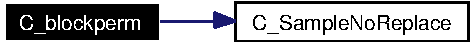
\includegraphics[width=131pt]{Helpers_8c_7c6b9e02fb5bcf919c7823d497cab062_cgraph}
\end{center}
\end{figure}
\hypertarget{Helpers_8c_f7c710920d1496d23fdabad9b1d0e18c}{
\index{Helpers.c@{Helpers.c}!C\_\-SampleNoReplace@{C\_\-SampleNoReplace}}
\index{C\_\-SampleNoReplace@{C\_\-SampleNoReplace}!Helpers.c@{Helpers.c}}
\subsubsection[{C\_\-SampleNoReplace}]{\setlength{\rightskip}{0pt plus 5cm}void C\_\-SampleNoReplace (int $\ast$ {\em x}, \/  int {\em m}, \/  int {\em k}, \/  int $\ast$ {\em ans})}}
\label{Helpers_8c_f7c710920d1496d23fdabad9b1d0e18c}


compute a permutation of a (random subset of) 0:(m-1) \begin{Desc}
\item[Parameters:]
\begin{description}
\item[{\em x}]an integer vector of length m \item[{\em m}]integer \item[{\em k}]integer \item[{\em ans}]an integer vector of length k \end{description}
\end{Desc}


Definition at line 42 of file Helpers.c.

Referenced by C\_\-blockperm().\hypertarget{Helpers_8c_f1f46cc3e98630497a1ccb21d943fe65}{
\index{Helpers.c@{Helpers.c}!ncol@{ncol}}
\index{ncol@{ncol}!Helpers.c@{Helpers.c}}
\subsubsection[{ncol}]{\setlength{\rightskip}{0pt plus 5cm}int ncol (SEXP {\em x})}}
\label{Helpers_8c_f1f46cc3e98630497a1ccb21d943fe65}




Definition at line 22 of file Helpers.c.

Referenced by R\_\-ExpectCovarInfluence(), R\_\-ExpectCovarLinearStatistic(), R\_\-kronecker(), R\_\-LinearStatistic(), R\_\-MonteCarloIndependenceTest(), and R\_\-PermutedLinearStatistic().\hypertarget{Helpers_8c_eeb672a71c45ead28b7b354414f2427a}{
\index{Helpers.c@{Helpers.c}!nrow@{nrow}}
\index{nrow@{nrow}!Helpers.c@{Helpers.c}}
\subsubsection[{nrow}]{\setlength{\rightskip}{0pt plus 5cm}int nrow (SEXP {\em x})}}
\label{Helpers_8c_eeb672a71c45ead28b7b354414f2427a}




Definition at line 11 of file Helpers.c.

Referenced by R\_\-ExpectCovarInfluence(), R\_\-ExpectCovarLinearStatistic(), R\_\-kronecker(), R\_\-LinearStatistic(), R\_\-MonteCarloIndependenceTest(), and R\_\-PermutedLinearStatistic().\hypertarget{Helpers_8c_c97588ec77f215433b2933e5632f810d}{
\index{Helpers.c@{Helpers.c}!R\_\-blockperm@{R\_\-blockperm}}
\index{R\_\-blockperm@{R\_\-blockperm}!Helpers.c@{Helpers.c}}
\subsubsection[{R\_\-blockperm}]{\setlength{\rightskip}{0pt plus 5cm}SEXP R\_\-blockperm (SEXP {\em block})}}
\label{Helpers_8c_c97588ec77f215433b2933e5632f810d}




Definition at line 139 of file Helpers.c.

References C\_\-blockperm(), and R\_\-blocksetup().

Here is the call graph for this function:\nopagebreak
\begin{figure}[H]
\begin{center}
\leavevmode
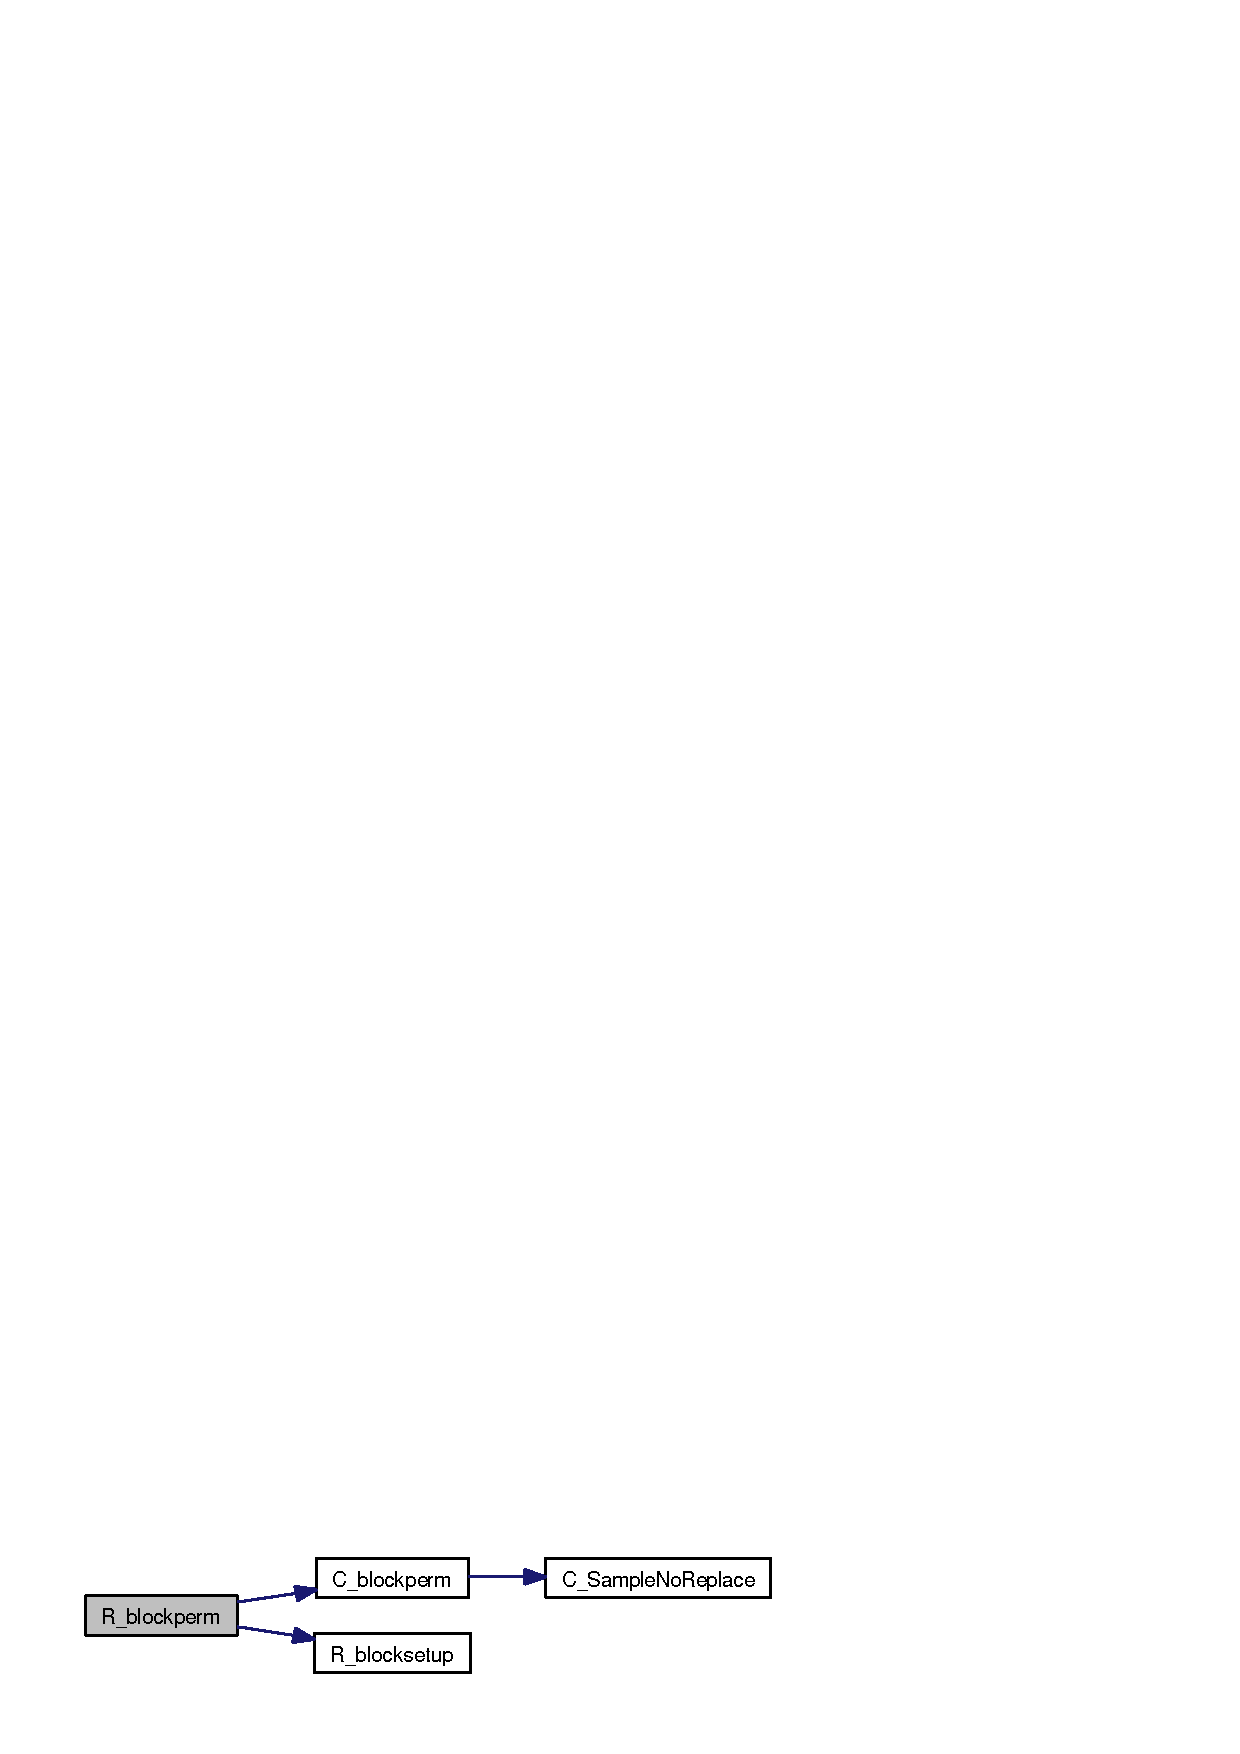
\includegraphics[width=187pt]{Helpers_8c_c97588ec77f215433b2933e5632f810d_cgraph}
\end{center}
\end{figure}
\hypertarget{Helpers_8c_877d7b2378274b833a8c14b27d7a16a1}{
\index{Helpers.c@{Helpers.c}!R\_\-blocksetup@{R\_\-blocksetup}}
\index{R\_\-blocksetup@{R\_\-blocksetup}!Helpers.c@{Helpers.c}}
\subsubsection[{R\_\-blocksetup}]{\setlength{\rightskip}{0pt plus 5cm}SEXP R\_\-blocksetup (SEXP {\em block})}}
\label{Helpers_8c_877d7b2378274b833a8c14b27d7a16a1}




Definition at line 56 of file Helpers.c.

Referenced by R\_\-blockperm(), and R\_\-MonteCarloIndependenceTest().\hypertarget{Helpers_8c_712dc63828d311dc3be30182fccf6f0f}{
\index{Helpers.c@{Helpers.c}!R\_\-maxstattrafo@{R\_\-maxstattrafo}}
\index{R\_\-maxstattrafo@{R\_\-maxstattrafo}!Helpers.c@{Helpers.c}}
\subsubsection[{R\_\-maxstattrafo}]{\setlength{\rightskip}{0pt plus 5cm}SEXP R\_\-maxstattrafo (SEXP {\em x}, \/  SEXP {\em cutpoints})}}
\label{Helpers_8c_712dc63828d311dc3be30182fccf6f0f}




Definition at line 204 of file Helpers.c.\hypertarget{Helpers_8c_140f9859faf864060c8a8ae129bc0190}{
\index{Helpers.c@{Helpers.c}!R\_\-MonteCarloIndependenceTest@{R\_\-MonteCarloIndependenceTest}}
\index{R\_\-MonteCarloIndependenceTest@{R\_\-MonteCarloIndependenceTest}!Helpers.c@{Helpers.c}}
\subsubsection[{R\_\-MonteCarloIndependenceTest}]{\setlength{\rightskip}{0pt plus 5cm}SEXP R\_\-MonteCarloIndependenceTest (SEXP {\em x}, \/  SEXP {\em y}, \/  SEXP {\em block}, \/  SEXP {\em B})}}
\label{Helpers_8c_140f9859faf864060c8a8ae129bc0190}




Definition at line 152 of file Helpers.c.

References C\_\-blockperm(), C\_\-PermutedLinearStatistic(), ncol(), nrow(), and R\_\-blocksetup().

Here is the call graph for this function:\nopagebreak
\begin{figure}[H]
\begin{center}
\leavevmode
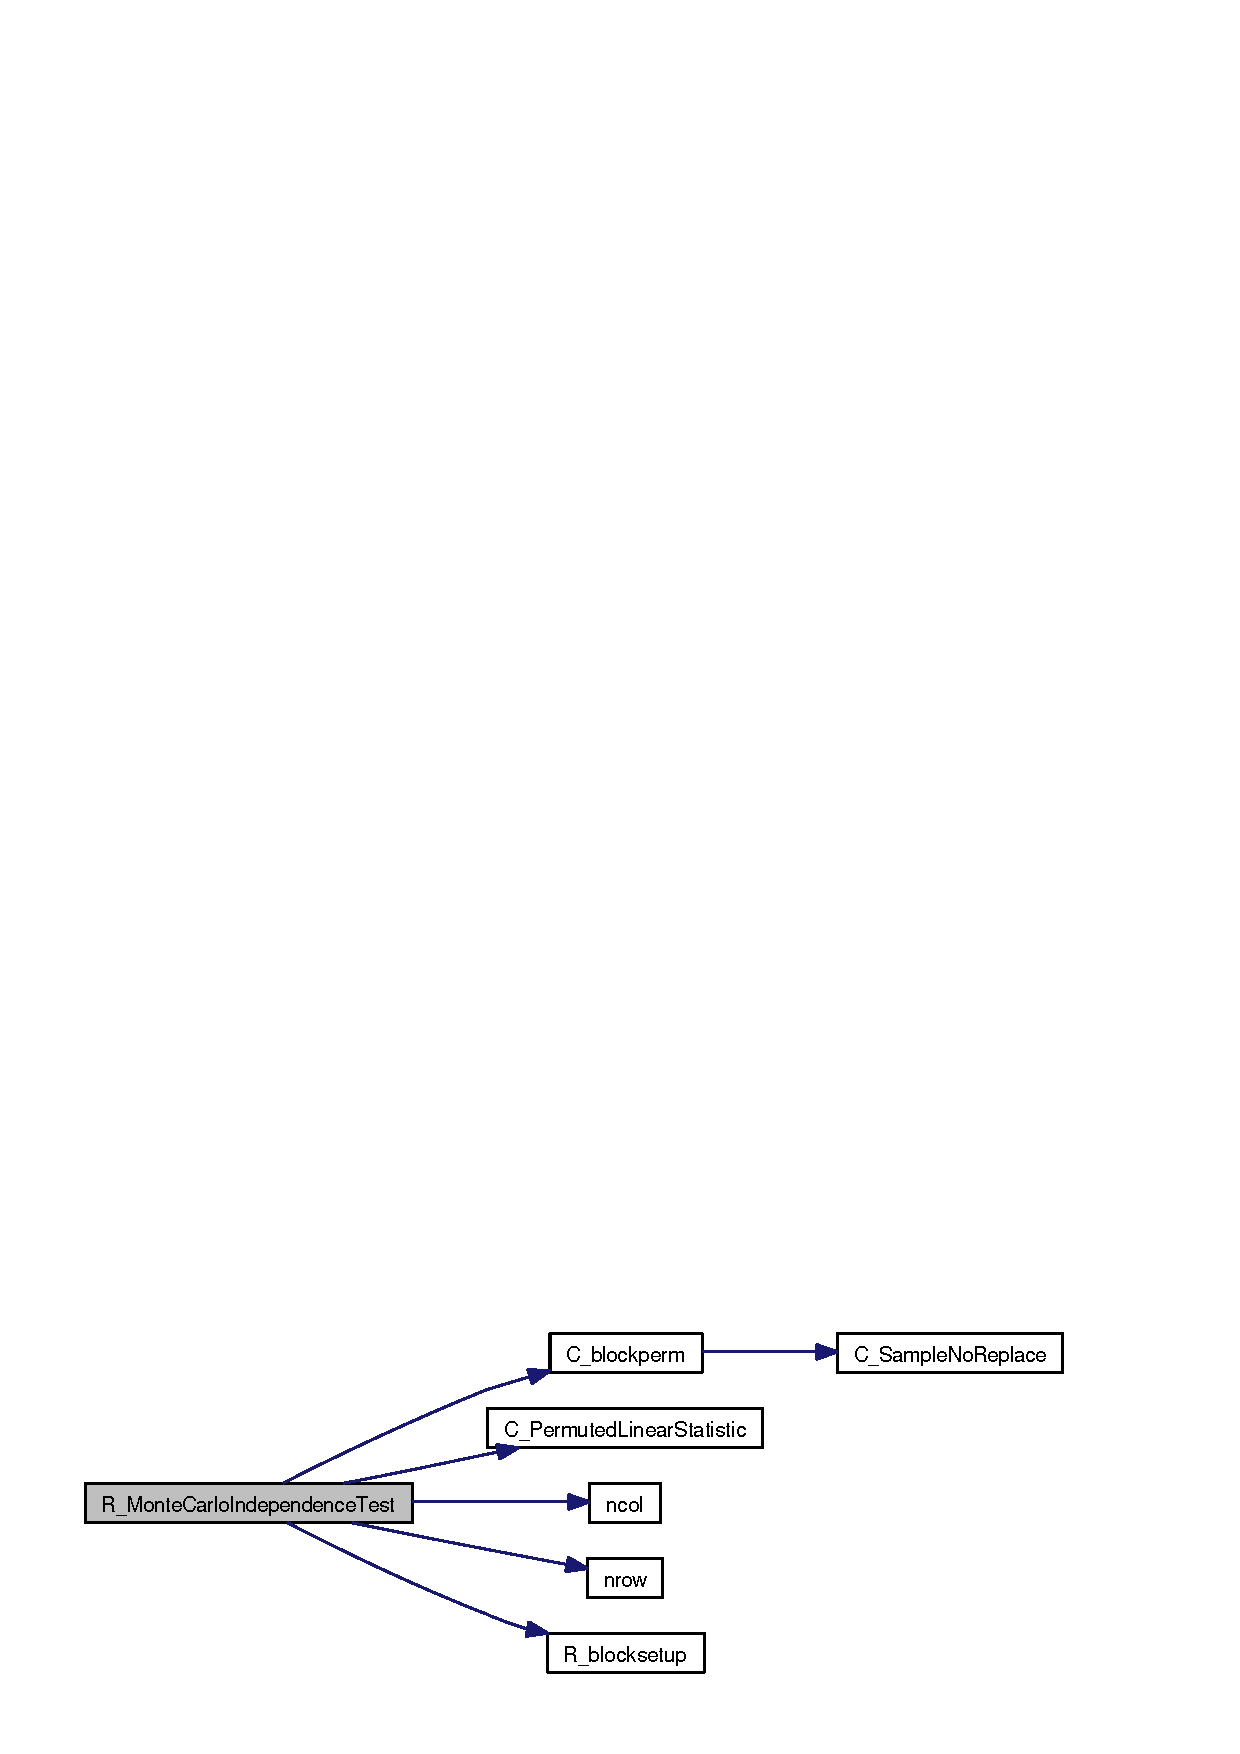
\includegraphics[width=257pt]{Helpers_8c_140f9859faf864060c8a8ae129bc0190_cgraph}
\end{center}
\end{figure}

\hypertarget{Helpers_8h}{
\section{Helpers.h File Reference}
\label{Helpers_8h}\index{Helpers.h@{Helpers.h}}
}


This graph shows which files directly or indirectly include this file:\begin{figure}[H]
\begin{center}
\leavevmode
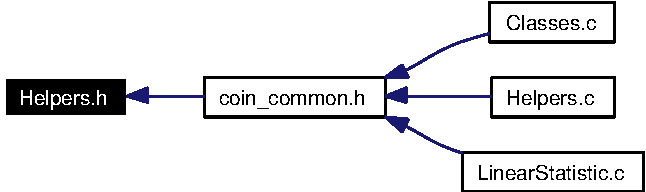
\includegraphics[width=172pt]{Helpers_8h__dep__incl}
\end{center}
\end{figure}
\subsection*{Functions}
\begin{CompactItemize}
\item 
int \hyperlink{Helpers_8h_eeb672a71c45ead28b7b354414f2427a}{nrow} (SEXP x)
\item 
int \hyperlink{Helpers_8h_f1f46cc3e98630497a1ccb21d943fe65}{ncol} (SEXP x)
\end{CompactItemize}


\subsection{Function Documentation}
\hypertarget{Helpers_8h_f1f46cc3e98630497a1ccb21d943fe65}{
\index{Helpers.h@{Helpers.h}!ncol@{ncol}}
\index{ncol@{ncol}!Helpers.h@{Helpers.h}}
\subsubsection[ncol]{\setlength{\rightskip}{0pt plus 5cm}int ncol (SEXP {\em x})}}
\label{Helpers_8h_f1f46cc3e98630497a1ccb21d943fe65}




Definition at line 22 of file Helpers.c.

Referenced by R\_\-Expect\-Covar\-Influence(), R\_\-Expect\-Covar\-Linear\-Statistic(), R\_\-kronecker(), R\_\-Linear\-Statistic(), and R\_\-Monte\-Carlo\-Independence\-Test().\hypertarget{Helpers_8h_eeb672a71c45ead28b7b354414f2427a}{
\index{Helpers.h@{Helpers.h}!nrow@{nrow}}
\index{nrow@{nrow}!Helpers.h@{Helpers.h}}
\subsubsection[nrow]{\setlength{\rightskip}{0pt plus 5cm}int nrow (SEXP {\em x})}}
\label{Helpers_8h_eeb672a71c45ead28b7b354414f2427a}




Definition at line 11 of file Helpers.c.

Referenced by R\_\-Expect\-Covar\-Influence(), R\_\-Expect\-Covar\-Linear\-Statistic(), R\_\-kronecker(), R\_\-Linear\-Statistic(), R\_\-Monte\-Carlo\-Independence\-Test(), and R\_\-Permuted\-Linear\-Statistic().
\hypertarget{LinearStatistic_8c}{
\section{Linear\-Statistic.c File Reference}
\label{LinearStatistic_8c}\index{LinearStatistic.c@{LinearStatistic.c}}
}
{\tt \#include \char`\"{}coin\_\-common.h\char`\"{}}\par


Include dependency graph for Linear\-Statistic.c:\begin{figure}[H]
\begin{center}
\leavevmode
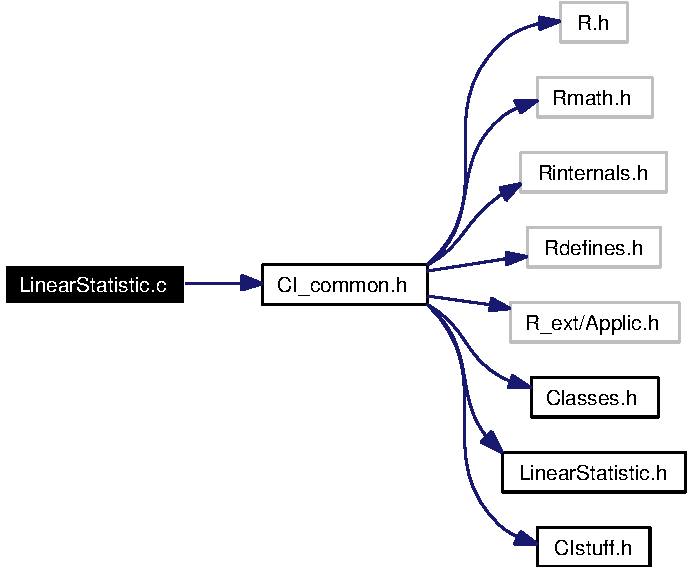
\includegraphics[width=186pt]{LinearStatistic_8c__incl}
\end{center}
\end{figure}
\subsection*{Functions}
\begin{CompactItemize}
\item 
void \hyperlink{LinearStatistic_8c_12e882779ecd0445c3a0dd9ac85dfeee}{C\_\-kronecker} (const double $\ast$A, const int m, const int n, const double $\ast$B, const int r, const int s, double $\ast$ans)
\item 
SEXP \hyperlink{LinearStatistic_8c_95f5ed4c75d42e2e98ed09c9c9d48ff5}{R\_\-kronecker} (SEXP A, SEXP B)
\item 
void \hyperlink{LinearStatistic_8c_e2f62abe13ee5b625141b5d4a496d832}{C\_\-Expect\-Covar\-Influence} (const double $\ast$y, const int q, const double $\ast$weights, const int n, SEXP ans)
\item 
SEXP \hyperlink{LinearStatistic_8c_6216ea560644c08002fb32756ae67dcc}{R\_\-Expect\-Covar\-Influence} (SEXP y, SEXP weights)
\item 
void \hyperlink{LinearStatistic_8c_94a0805ea258af79d426c095feee399a}{C\_\-Expect\-Covar\-Linear\-Statistic} (const double $\ast$x, const int p, const double $\ast$y, const int q, const double $\ast$weights, const int n, const SEXP expcovinf, SEXP ans)
\item 
SEXP \hyperlink{LinearStatistic_8c_58fff8082d3ab197994a21a10c422353}{R\_\-Expect\-Covar\-Linear\-Statistic} (SEXP x, SEXP y, SEXP weights, SEXP expcovinf)
\item 
void \hyperlink{LinearStatistic_8c_aefa2a9406bb30b323715e3db41da637}{C\_\-Linear\-Statistic} (const double $\ast$x, const int p, const double $\ast$y, const int q, const double $\ast$weights, const int n, double $\ast$ans)
\item 
SEXP \hyperlink{LinearStatistic_8c_732bfc8e1797d8953482aa31f9b43e5f}{R\_\-Linear\-Statistic} (SEXP x, SEXP y, SEXP weights)
\item 
void \hyperlink{LinearStatistic_8c_a34b0f12fac36231a105d6dc903bfe89}{C\_\-Permuted\-Linear\-Statistic} (const double $\ast$x, const int p, const double $\ast$y, const int q, const int n, const int nperm, const int $\ast$indx, const int $\ast$perm, double $\ast$ans)
\item 
SEXP \hyperlink{LinearStatistic_8c_be383bcae17e8b3a1d5740ec16a9817a}{R\_\-Permuted\-Linear\-Statistic} (SEXP x, SEXP y, SEXP indx, SEXP perm)
\end{CompactItemize}


\subsection{Detailed Description}
Linear statistics for conditional inference

\begin{Desc}
\item[Author:]\begin{Desc}
\item[Author]hothorn \end{Desc}
\end{Desc}
\begin{Desc}
\item[Date:]\begin{Desc}
\item[Date]2007-02-15 09:25:46 +0100 (Thu, 15 Feb 2007) \end{Desc}
\end{Desc}


Definition in file \hyperlink{LinearStatistic_8c-source}{Linear\-Statistic.c}.

\subsection{Function Documentation}
\hypertarget{LinearStatistic_8c_e2f62abe13ee5b625141b5d4a496d832}{
\index{LinearStatistic.c@{Linear\-Statistic.c}!C_ExpectCovarInfluence@{C\_\-ExpectCovarInfluence}}
\index{C_ExpectCovarInfluence@{C\_\-ExpectCovarInfluence}!LinearStatistic.c@{Linear\-Statistic.c}}
\subsubsection[C\_\-ExpectCovarInfluence]{\setlength{\rightskip}{0pt plus 5cm}void C\_\-Expect\-Covar\-Influence (const double $\ast$ {\em y}, const int {\em q}, const double $\ast$ {\em weights}, const int {\em n}, SEXP {\em ans})}}
\label{LinearStatistic_8c_e2f62abe13ee5b625141b5d4a496d832}


Conditional expectation and covariance of the influence function\par
 \begin{Desc}
\item[Parameters:]
\begin{description}
\item[{\em y}]values of the influence function \item[{\em q}]dimension of the influence function \item[{\em weights}]case weights \item[{\em n}]number of observations \item[{\em ans}]return value; an object of class `Expect\-Covar\-Influence' \end{description}
\end{Desc}


Definition at line 80 of file Linear\-Statistic.c.

References coin\_\-covariance\-Sym, coin\_\-expectation\-Sym, and coin\_\-sumweights\-Sym.

Referenced by R\_\-Expect\-Covar\-Influence().\hypertarget{LinearStatistic_8c_94a0805ea258af79d426c095feee399a}{
\index{LinearStatistic.c@{Linear\-Statistic.c}!C_ExpectCovarLinearStatistic@{C\_\-ExpectCovarLinearStatistic}}
\index{C_ExpectCovarLinearStatistic@{C\_\-ExpectCovarLinearStatistic}!LinearStatistic.c@{Linear\-Statistic.c}}
\subsubsection[C\_\-ExpectCovarLinearStatistic]{\setlength{\rightskip}{0pt plus 5cm}void C\_\-Expect\-Covar\-Linear\-Statistic (const double $\ast$ {\em x}, const int {\em p}, const double $\ast$ {\em y}, const int {\em q}, const double $\ast$ {\em weights}, const int {\em n}, const SEXP {\em expcovinf}, SEXP {\em ans})}}
\label{LinearStatistic_8c_94a0805ea258af79d426c095feee399a}


Conditional expectation and covariance of the a linear statistic\par
 \begin{Desc}
\item[Parameters:]
\begin{description}
\item[{\em x}]values of the transformation \item[{\em p}]dimension of the transformation \item[{\em y}]values of the influence function \item[{\em q}]dimension of the influence function \item[{\em weights}]case weights \item[{\em n}]number of observations \item[{\em expcovinf}]an object of class `Expect\-Covar\-Influence' \item[{\em ans}]return value; an object of class `Expect\-Covar' \end{description}
\end{Desc}


Definition at line 192 of file Linear\-Statistic.c.

References coin\_\-covariance\-Sym, coin\_\-expectation\-Sym, and coin\_\-sumweights\-Sym.

Referenced by R\_\-Expect\-Covar\-Linear\-Statistic().\hypertarget{LinearStatistic_8c_12e882779ecd0445c3a0dd9ac85dfeee}{
\index{LinearStatistic.c@{Linear\-Statistic.c}!C_kronecker@{C\_\-kronecker}}
\index{C_kronecker@{C\_\-kronecker}!LinearStatistic.c@{Linear\-Statistic.c}}
\subsubsection[C\_\-kronecker]{\setlength{\rightskip}{0pt plus 5cm}void C\_\-kronecker (const double $\ast$ {\em A}, const int {\em m}, const int {\em n}, const double $\ast$ {\em B}, const int {\em r}, const int {\em s}, double $\ast$ {\em ans})}}
\label{LinearStatistic_8c_12e882779ecd0445c3a0dd9ac85dfeee}


Computes the Kronecker product of two matrices\par
 \begin{Desc}
\item[Parameters:]
\begin{description}
\item[{\em A}]matrix \item[{\em m}]nrow(A) \item[{\em n}]ncol(A) \item[{\em B}]matrix \item[{\em r}]nrow(B) \item[{\em s}]ncol(B) \item[{\em ans}]return value; a pointer to a REALSXP-vector of length (mr x ns) \end{description}
\end{Desc}


Definition at line 22 of file Linear\-Statistic.c.

Referenced by R\_\-kronecker().\hypertarget{LinearStatistic_8c_aefa2a9406bb30b323715e3db41da637}{
\index{LinearStatistic.c@{Linear\-Statistic.c}!C_LinearStatistic@{C\_\-LinearStatistic}}
\index{C_LinearStatistic@{C\_\-LinearStatistic}!LinearStatistic.c@{Linear\-Statistic.c}}
\subsubsection[C\_\-LinearStatistic]{\setlength{\rightskip}{0pt plus 5cm}void C\_\-Linear\-Statistic (const double $\ast$ {\em x}, const int {\em p}, const double $\ast$ {\em y}, const int {\em q}, const double $\ast$ {\em weights}, const int {\em n}, double $\ast$ {\em ans})}}
\label{LinearStatistic_8c_aefa2a9406bb30b323715e3db41da637}


Computes the linear statistic, formula (1) in the paper\par
 \begin{Desc}
\item[Parameters:]
\begin{description}
\item[{\em x}]values of the transformation \item[{\em p}]dimension of the transformation \item[{\em y}]values of the influence function \item[{\em q}]dimension of the influence function \item[{\em weights}]case weights \item[{\em n}]number of observations \item[{\em ans}]return value; a pointer to a REALSXP-vector of length pq \end{description}
\end{Desc}


Definition at line 327 of file Linear\-Statistic.c.

Referenced by R\_\-Linear\-Statistic().\hypertarget{LinearStatistic_8c_a34b0f12fac36231a105d6dc903bfe89}{
\index{LinearStatistic.c@{Linear\-Statistic.c}!C_PermutedLinearStatistic@{C\_\-PermutedLinearStatistic}}
\index{C_PermutedLinearStatistic@{C\_\-PermutedLinearStatistic}!LinearStatistic.c@{Linear\-Statistic.c}}
\subsubsection[C\_\-PermutedLinearStatistic]{\setlength{\rightskip}{0pt plus 5cm}void C\_\-Permuted\-Linear\-Statistic (const double $\ast$ {\em x}, const int {\em p}, const double $\ast$ {\em y}, const int {\em q}, const int {\em n}, const int {\em nperm}, const int $\ast$ {\em indx}, const int $\ast$ {\em perm}, double $\ast$ {\em ans})}}
\label{LinearStatistic_8c_a34b0f12fac36231a105d6dc903bfe89}


Linear Statistic with permuted indices\par
 \begin{Desc}
\item[Parameters:]
\begin{description}
\item[{\em x}]values of the transformation \item[{\em p}]dimension of the transformation \item[{\em y}]values of the influence function \item[{\em q}]dimension of the influence function \item[{\em n}]number of observations \item[{\em nperm}]number of permutations \item[{\em indx}]indices for the x-part \item[{\em perm}](permuted) indices for the y-part \item[{\em ans}]return value; a pointer to a REALSXP-vector of length pq \end{description}
\end{Desc}


Definition at line 409 of file Linear\-Statistic.c.

Referenced by R\_\-Monte\-Carlo\-Independence\-Test().\hypertarget{LinearStatistic_8c_6216ea560644c08002fb32756ae67dcc}{
\index{LinearStatistic.c@{Linear\-Statistic.c}!R_ExpectCovarInfluence@{R\_\-ExpectCovarInfluence}}
\index{R_ExpectCovarInfluence@{R\_\-ExpectCovarInfluence}!LinearStatistic.c@{Linear\-Statistic.c}}
\subsubsection[R\_\-ExpectCovarInfluence]{\setlength{\rightskip}{0pt plus 5cm}SEXP R\_\-Expect\-Covar\-Influence (SEXP {\em y}, SEXP {\em weights})}}
\label{LinearStatistic_8c_6216ea560644c08002fb32756ae67dcc}


R-interface to C\_\-Expect\-Covar\-Influence\par
 \begin{Desc}
\item[Parameters:]
\begin{description}
\item[{\em y}]values of the influence function \item[{\em weights}]case weights \end{description}
\end{Desc}


Definition at line 150 of file Linear\-Statistic.c.

References C\_\-Expect\-Covar\-Influence(), coin\_\-covariance\-Sym, coin\_\-expectation\-Sym, coin\_\-sumweights\-Sym, ncol(), and nrow().

Here is the call graph for this function:\begin{figure}[H]
\begin{center}
\leavevmode
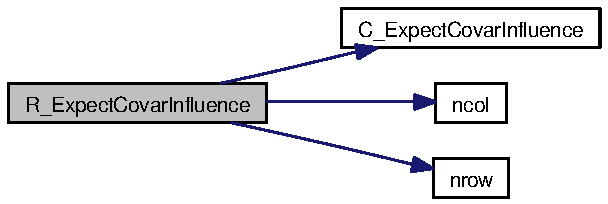
\includegraphics[width=164pt]{LinearStatistic_8c_6216ea560644c08002fb32756ae67dcc_cgraph}
\end{center}
\end{figure}
\hypertarget{LinearStatistic_8c_58fff8082d3ab197994a21a10c422353}{
\index{LinearStatistic.c@{Linear\-Statistic.c}!R_ExpectCovarLinearStatistic@{R\_\-ExpectCovarLinearStatistic}}
\index{R_ExpectCovarLinearStatistic@{R\_\-ExpectCovarLinearStatistic}!LinearStatistic.c@{Linear\-Statistic.c}}
\subsubsection[R\_\-ExpectCovarLinearStatistic]{\setlength{\rightskip}{0pt plus 5cm}SEXP R\_\-Expect\-Covar\-Linear\-Statistic (SEXP {\em x}, SEXP {\em y}, SEXP {\em weights}, SEXP {\em expcovinf})}}
\label{LinearStatistic_8c_58fff8082d3ab197994a21a10c422353}


R-interface to C\_\-Expect\-Covar\-Linear\-Statistic\par
 \begin{Desc}
\item[Parameters:]
\begin{description}
\item[{\em x}]values of the transformation \item[{\em y}]values of the influence function \item[{\em weights}]case weights \item[{\em expcovinf}]an object of class `Expect\-Covar\-Influence' \end{description}
\end{Desc}


Definition at line 285 of file Linear\-Statistic.c.

References C\_\-Expect\-Covar\-Linear\-Statistic(), coin\_\-covariance\-Sym, coin\_\-expectation\-Sym, ncol(), and nrow().

Here is the call graph for this function:\begin{figure}[H]
\begin{center}
\leavevmode
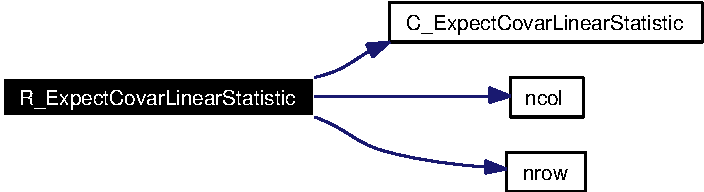
\includegraphics[width=186pt]{LinearStatistic_8c_58fff8082d3ab197994a21a10c422353_cgraph}
\end{center}
\end{figure}
\hypertarget{LinearStatistic_8c_95f5ed4c75d42e2e98ed09c9c9d48ff5}{
\index{LinearStatistic.c@{Linear\-Statistic.c}!R_kronecker@{R\_\-kronecker}}
\index{R_kronecker@{R\_\-kronecker}!LinearStatistic.c@{Linear\-Statistic.c}}
\subsubsection[R\_\-kronecker]{\setlength{\rightskip}{0pt plus 5cm}SEXP R\_\-kronecker (SEXP {\em A}, SEXP {\em B})}}
\label{LinearStatistic_8c_95f5ed4c75d42e2e98ed09c9c9d48ff5}


R-interface to C\_\-kronecker\par
 \begin{Desc}
\item[Parameters:]
\begin{description}
\item[{\em A}]matrix \item[{\em B}]matrix \end{description}
\end{Desc}


Definition at line 51 of file Linear\-Statistic.c.

References C\_\-kronecker(), ncol(), and nrow().

Here is the call graph for this function:\begin{figure}[H]
\begin{center}
\leavevmode
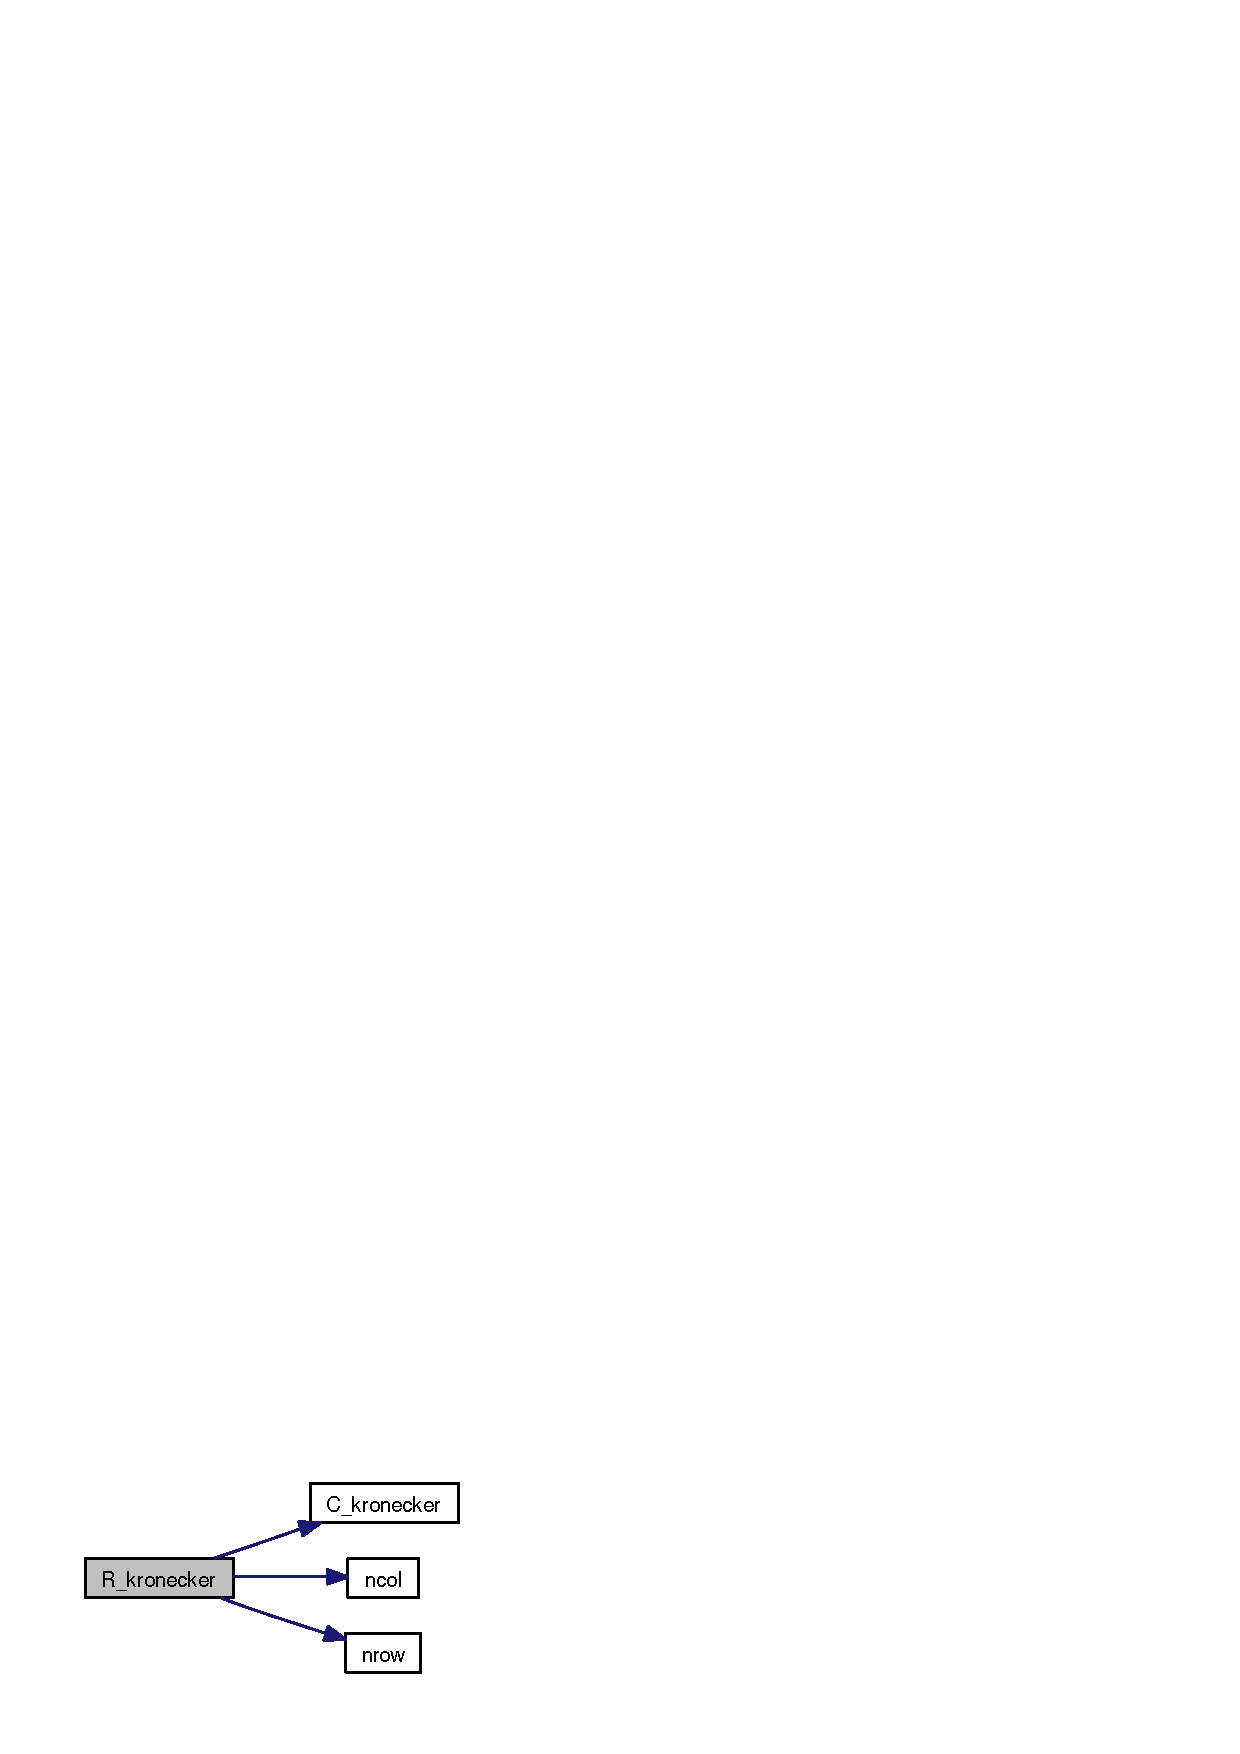
\includegraphics[width=110pt]{LinearStatistic_8c_95f5ed4c75d42e2e98ed09c9c9d48ff5_cgraph}
\end{center}
\end{figure}
\hypertarget{LinearStatistic_8c_732bfc8e1797d8953482aa31f9b43e5f}{
\index{LinearStatistic.c@{Linear\-Statistic.c}!R_LinearStatistic@{R\_\-LinearStatistic}}
\index{R_LinearStatistic@{R\_\-LinearStatistic}!LinearStatistic.c@{Linear\-Statistic.c}}
\subsubsection[R\_\-LinearStatistic]{\setlength{\rightskip}{0pt plus 5cm}SEXP R\_\-Linear\-Statistic (SEXP {\em x}, SEXP {\em y}, SEXP {\em weights})}}
\label{LinearStatistic_8c_732bfc8e1797d8953482aa31f9b43e5f}


R-interface to C\_\-Linear\-Statistic \par
 \begin{Desc}
\item[Parameters:]
\begin{description}
\item[{\em x}]values of the transformation \item[{\em y}]values of the influence function \item[{\em weights}]case weights \end{description}
\end{Desc}


Definition at line 363 of file Linear\-Statistic.c.

References C\_\-Linear\-Statistic(), ncol(), and nrow().

Here is the call graph for this function:\begin{figure}[H]
\begin{center}
\leavevmode
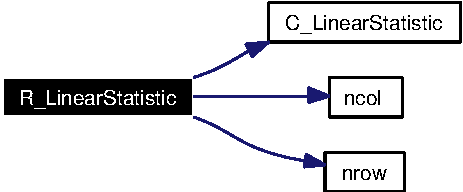
\includegraphics[width=128pt]{LinearStatistic_8c_732bfc8e1797d8953482aa31f9b43e5f_cgraph}
\end{center}
\end{figure}
\hypertarget{LinearStatistic_8c_be383bcae17e8b3a1d5740ec16a9817a}{
\index{LinearStatistic.c@{Linear\-Statistic.c}!R_PermutedLinearStatistic@{R\_\-PermutedLinearStatistic}}
\index{R_PermutedLinearStatistic@{R\_\-PermutedLinearStatistic}!LinearStatistic.c@{Linear\-Statistic.c}}
\subsubsection[R\_\-PermutedLinearStatistic]{\setlength{\rightskip}{0pt plus 5cm}SEXP R\_\-Permuted\-Linear\-Statistic (SEXP {\em x}, SEXP {\em y}, SEXP {\em indx}, SEXP {\em perm})}}
\label{LinearStatistic_8c_be383bcae17e8b3a1d5740ec16a9817a}


Linear Statistic with permuted indices\par
 \begin{Desc}
\item[Parameters:]
\begin{description}
\item[{\em x}]values of the transformation \item[{\em y}]values of the influence function \item[{\em indx}]indices for the x-part \item[{\em perm}](permuted) indices for the y-part \end{description}
\end{Desc}


Definition at line 442 of file Linear\-Statistic.c.

References nrow().

Here is the call graph for this function:\begin{figure}[H]
\begin{center}
\leavevmode
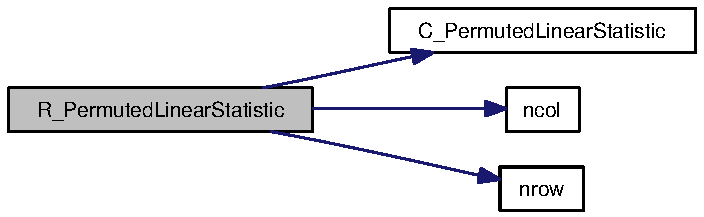
\includegraphics[width=123pt]{LinearStatistic_8c_be383bcae17e8b3a1d5740ec16a9817a_cgraph}
\end{center}
\end{figure}

\hypertarget{LinearStatistic_8h}{
\section{Linear\-Statistic.h File Reference}
\label{LinearStatistic_8h}\index{LinearStatistic.h@{LinearStatistic.h}}
}


This graph shows which files directly or indirectly include this file:\begin{figure}[H]
\begin{center}
\leavevmode
\includegraphics[width=182pt]{LinearStatistic_8h__dep__incl}
\end{center}
\end{figure}
\subsection*{Functions}
\begin{CompactItemize}
\item 
void \hyperlink{LinearStatistic_8h_a34b0f12fac36231a105d6dc903bfe89}{C\_\-Permuted\-Linear\-Statistic} (const double $\ast$x, const int p, const double $\ast$y, const int q, const int n, const int nperm, const int $\ast$indx, const int $\ast$perm, double $\ast$ans)
\end{CompactItemize}


\subsection{Function Documentation}
\hypertarget{LinearStatistic_8h_a34b0f12fac36231a105d6dc903bfe89}{
\index{LinearStatistic.h@{Linear\-Statistic.h}!C_PermutedLinearStatistic@{C\_\-PermutedLinearStatistic}}
\index{C_PermutedLinearStatistic@{C\_\-PermutedLinearStatistic}!LinearStatistic.h@{Linear\-Statistic.h}}
\subsubsection[C\_\-PermutedLinearStatistic]{\setlength{\rightskip}{0pt plus 5cm}void C\_\-Permuted\-Linear\-Statistic (const double $\ast$ {\em x}, const int {\em p}, const double $\ast$ {\em y}, const int {\em q}, const int {\em n}, const int {\em nperm}, const int $\ast$ {\em indx}, const int $\ast$ {\em perm}, double $\ast$ {\em ans})}}
\label{LinearStatistic_8h_a34b0f12fac36231a105d6dc903bfe89}


Linear Statistic with permuted indices\par
 \begin{Desc}
\item[Parameters:]
\begin{description}
\item[{\em x}]values of the transformation \item[{\em p}]dimension of the transformation \item[{\em y}]values of the influence function \item[{\em q}]dimension of the influence function \item[{\em n}]number of observations \item[{\em nperm}]number of permutations \item[{\em indx}]indices for the x-part \item[{\em perm}](permuted) indices for the y-part \item[{\em ans}]return value; a pointer to a REALSXP-vector of length pq \end{description}
\end{Desc}


Definition at line 409 of file Linear\-Statistic.c.

Referenced by R\_\-Monte\-Carlo\-Independence\-Test().
\hypertarget{StreitbergRoehmel_8c}{
\section{StreitbergRoehmel.c File Reference}
\label{StreitbergRoehmel_8c}\index{StreitbergRoehmel.c@{StreitbergRoehmel.c}}
}
{\tt \#include $<$R.h$>$}\par
{\tt \#include $<$Rmath.h$>$}\par
{\tt \#include $<$Rdefines.h$>$}\par


Include dependency graph for StreitbergRoehmel.c:\nopagebreak
\begin{figure}[H]
\begin{center}
\leavevmode
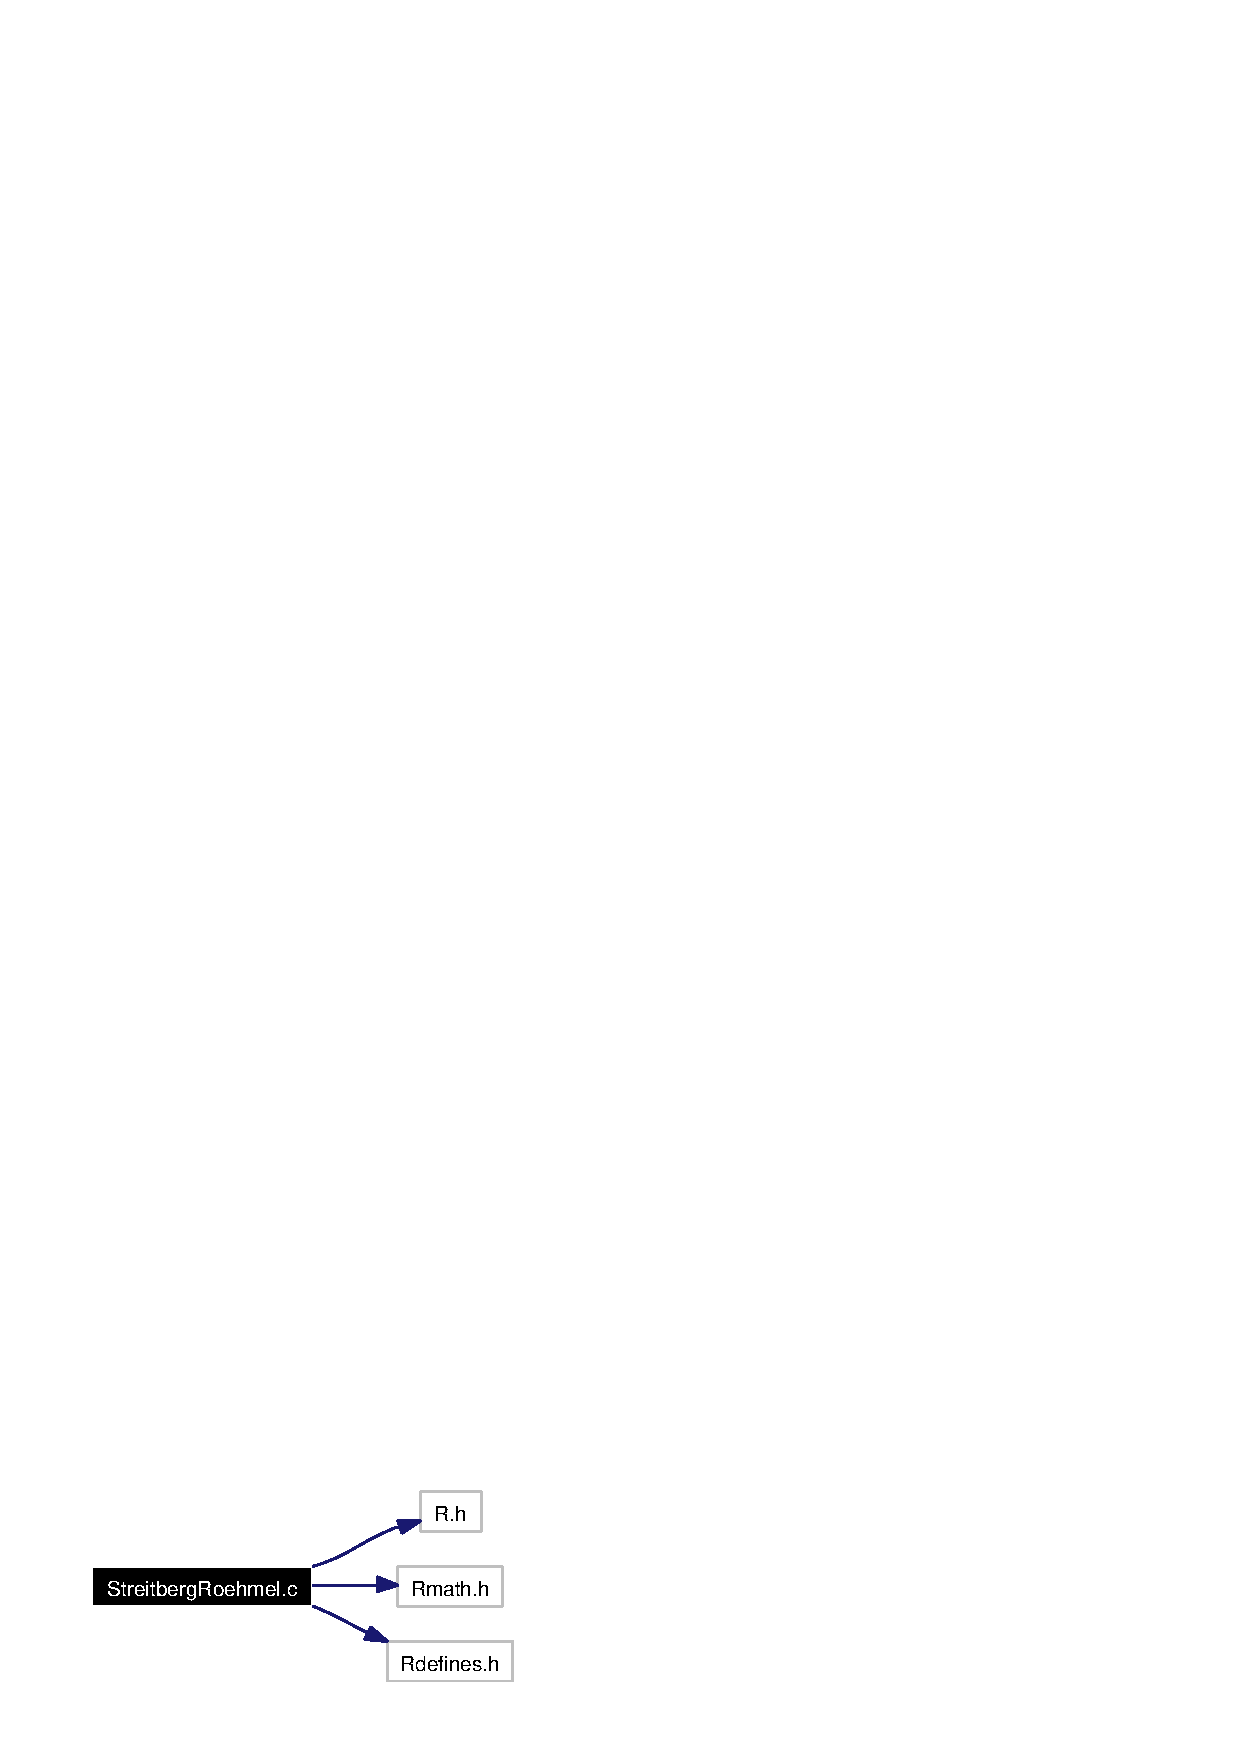
\includegraphics[width=112pt]{StreitbergRoehmel_8c__incl}
\end{center}
\end{figure}
\subsection*{Functions}
\begin{CompactItemize}
\item 
SEXP \hyperlink{StreitbergRoehmel_8c_f9a845b0ec4e288550ee071a11d42e3f}{R\_\-cpermdist2} (SEXP score\_\-a, SEXP score\_\-b, SEXP m\_\-a, SEXP m\_\-b, SEXP retProb)
\item 
SEXP \hyperlink{StreitbergRoehmel_8c_5bccf6c77bf2cabd9930b24d7fac273a}{R\_\-cpermdist1} (SEXP scores)
\end{CompactItemize}


\subsection{Detailed Description}
Exact Distribution of Two-Sample Permutation Tests Streitberg \& Roehmel Algorithm

\begin{Desc}
\item[Author:]\end{Desc}
\begin{Desc}
\item[Author]hothorn \end{Desc}
\begin{Desc}
\item[Date:]\end{Desc}
\begin{Desc}
\item[Date]2007-07-18 18:29:22 +0200 (Wed, 18 Jul 2007) \end{Desc}


Definition in file \hyperlink{StreitbergRoehmel_8c-source}{StreitbergRoehmel.c}.

\subsection{Function Documentation}
\hypertarget{StreitbergRoehmel_8c_5bccf6c77bf2cabd9930b24d7fac273a}{
\index{StreitbergRoehmel.c@{StreitbergRoehmel.c}!R\_\-cpermdist1@{R\_\-cpermdist1}}
\index{R\_\-cpermdist1@{R\_\-cpermdist1}!StreitbergRoehmel.c@{StreitbergRoehmel.c}}
\subsubsection[R\_\-cpermdist1]{\setlength{\rightskip}{0pt plus 5cm}SEXP R\_\-cpermdist1 (SEXP {\em scores})}}
\label{StreitbergRoehmel_8c_5bccf6c77bf2cabd9930b24d7fac273a}


The density of the permutation distribution for the one sample problem.

REFERENCES

Bernd Streitberg \& Joachim R$\backslash$\char`\"{}ohmel (1986), Exact distributions for permutations and rank tests: An introduction to some recently published algorithms. Statistical Software Newsletter 12(1), 10-17.

Bernd Streitberg \& Joachim R$\backslash$\char`\"{}ohmel (1987), Exakte Verteilungen f$\backslash$\char`\"{}ur Rang- und Randomisierungstests im allgemeinen \$c\$-Stichprobenfall. EDV in Medizin und Biologie 18(1), 12-19 (in german).

\begin{Desc}
\item[Parameters:]
\begin{description}
\item[{\em scores}]score vector (such as rank(abs(y)) for wilcoxsign\_\-test) \end{description}
\end{Desc}


Definition at line 198 of file StreitbergRoehmel.c.\hypertarget{StreitbergRoehmel_8c_f9a845b0ec4e288550ee071a11d42e3f}{
\index{StreitbergRoehmel.c@{StreitbergRoehmel.c}!R\_\-cpermdist2@{R\_\-cpermdist2}}
\index{R\_\-cpermdist2@{R\_\-cpermdist2}!StreitbergRoehmel.c@{StreitbergRoehmel.c}}
\subsubsection[R\_\-cpermdist2]{\setlength{\rightskip}{0pt plus 5cm}SEXP R\_\-cpermdist2 (SEXP {\em score\_\-a}, \/  SEXP {\em score\_\-b}, \/  SEXP {\em m\_\-a}, \/  SEXP {\em m\_\-b}, \/  SEXP {\em retProb})}}
\label{StreitbergRoehmel_8c_f9a845b0ec4e288550ee071a11d42e3f}


The density of the permutation distribution for the independent two sample problem.

REFERENCES

Bernd Streitberg \& Joachim R$\backslash$\char`\"{}ohmel (1986), Exact distributions for permutations and rank tests: An introduction to some recently published algorithms. Statistical Software Newsletter 12(1), 10-17.

Bernd Streitberg \& Joachim R$\backslash$\char`\"{}ohmel (1987), Exakte Verteilungen f$\backslash$\char`\"{}ur Rang- und Randomisierungstests im allgemeinen \$c\$-Stichprobenfall. EDV in Medizin und Biologie 18(1), 12-19 (in german).

\begin{Desc}
\item[Parameters:]
\begin{description}
\item[{\em score\_\-a}]score vector (typically c(1,1,...,1)) \item[{\em score\_\-b}]score vector (typically ranks) \item[{\em m\_\-a}]integer indicating the sum of m\_\-a elements of score\_\-a \item[{\em m\_\-b}]integer indicating the sum of m\_\-b elements of score\_\-b \item[{\em retProb}]logical indicating whether the density (TRUE) or the matrix of all permutations should be returned \end{description}
\end{Desc}


Definition at line 39 of file StreitbergRoehmel.c.
\hypertarget{vandeWiel_8c}{
\section{vandeWiel.c File Reference}
\label{vandeWiel_8c}\index{vandeWiel.c@{vandeWiel.c}}
}
{\tt \#include $<$R.h$>$}\par
{\tt \#include $<$Rmath.h$>$}\par
{\tt \#include $<$Rdefines.h$>$}\par


Include dependency graph for vandeWiel.c:\nopagebreak
\begin{figure}[H]
\begin{center}
\leavevmode
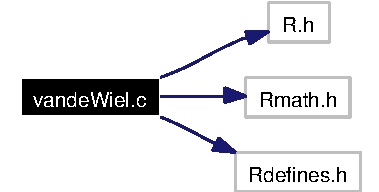
\includegraphics[width=112pt]{vandeWiel_8c__incl}
\end{center}
\end{figure}
\subsection*{Classes}
\begin{CompactItemize}
\item 
struct \hyperlink{structcelW}{celW}
\end{CompactItemize}
\subsection*{Functions}
\begin{CompactItemize}
\item 
double \hyperlink{vandeWiel_8c_dd09844ac40346e216f503f95e644970}{binomi} (int m, int n)
\item 
\hyperlink{structcelW}{celW} $\ast$$\ast$ \hyperlink{vandeWiel_8c_03d7f636d17008a6fbe230458a92ddba}{reserveW} (int a, int b)
\item 
void \hyperlink{vandeWiel_8c_f72cc4501998ae01067d5555382b1609}{FreeW} (int a, \hyperlink{structcelW}{celW} $\ast$$\ast$W)
\item 
void \hyperlink{vandeWiel_8c_402c3e72a2fa3d600d4a4e8ace9f040b}{initW} (int a, int b, \hyperlink{structcelW}{celW} $\ast$$\ast$W)
\item 
void \hyperlink{vandeWiel_8c_e1d7e7e209f5b99745c8bca03057f761}{mult} (\hyperlink{structcelW}{celW} $\ast$tem, int a, int b, int rank, double $\ast$rs)
\item 
void \hyperlink{vandeWiel_8c_965c6db84dd8be42e1313d8c3ef9a784}{plus} (\hyperlink{structcelW}{celW} $\ast$$\ast$W, \hyperlink{structcelW}{celW} $\ast$tempie, int a, int b)
\item 
void \hyperlink{vandeWiel_8c_2f117e88849518e50d7d0eef3af07bf0}{mymergesort} (\hyperlink{structcelW}{celW} temptw, long tijd)
\item 
void \hyperlink{vandeWiel_8c_59f513c0ee260be89ad37daacf49e7e8}{fillcell} (\hyperlink{structcelW}{celW} $\ast$$\ast$W, int i1, int j1, int r, double $\ast$rs)
\item 
void \hyperlink{vandeWiel_8c_d0195ffa22342dfadee0abeb564931dc}{mirrorW} (\hyperlink{structcelW}{celW} $\ast$$\ast$W, int ce, int bep, int start, double $\ast$rs)
\item 
void \hyperlink{vandeWiel_8c_fb521caca26031c6fa9e92450685f5d1}{makeW} (\hyperlink{structcelW}{celW} $\ast$$\ast$W, int a, int b, int start, double $\ast$rs)
\item 
void \hyperlink{vandeWiel_8c_76539410f65d0d4c5105bacf1b32f093}{cumulcoef} (\hyperlink{structcelW}{celW} $\ast$$\ast$W, int i1, int j1)
\item 
double \hyperlink{vandeWiel_8c_14307006f6d9ec07bdfce7e853665bc5}{numbersmall} (int c, int b, double ob, \hyperlink{structcelW}{celW} $\ast$$\ast$W1, \hyperlink{structcelW}{celW} $\ast$$\ast$W2)
\item 
SEXP \hyperlink{vandeWiel_8c_a50657b564a35ab41b3e3e50e62c51b1}{R\_\-split\_\-up\_\-2sample} (SEXP scores, SEXP m, SEXP obs)
\end{CompactItemize}


\subsection{Detailed Description}
Exact Distribution of Two-Sample Permutation Tests van de Wiel split-up Algorithm

Author: Mark van de Wiel (2001-2005) $<$\href{mailto:m.a.v.d.wiel@TUE.nl}{\tt m.a.v.d.wiel@TUE.nl}$>$ with modifications for R by Torsten Hothorn $<$\href{mailto:Torsten.Hothorn@R-project.org}{\tt Torsten.Hothorn@R-project.org}$>$

\begin{Desc}
\item[Author:]\end{Desc}
\begin{Desc}
\item[Author]hothorn \end{Desc}
\begin{Desc}
\item[Date:]\end{Desc}
\begin{Desc}
\item[Date]2005-07-28 17:04:29 +0200 (Thu, 28 Jul 2005) \end{Desc}


Definition in file \hyperlink{vandeWiel_8c-source}{vandeWiel.c}.

\subsection{Function Documentation}
\hypertarget{vandeWiel_8c_dd09844ac40346e216f503f95e644970}{
\index{vandeWiel.c@{vandeWiel.c}!binomi@{binomi}}
\index{binomi@{binomi}!vandeWiel.c@{vandeWiel.c}}
\subsubsection[{binomi}]{\setlength{\rightskip}{0pt plus 5cm}double binomi (int {\em m}, \/  int {\em n})}}
\label{vandeWiel_8c_dd09844ac40346e216f503f95e644970}




Definition at line 37 of file vandeWiel.c.

Referenced by R\_\-split\_\-up\_\-2sample(), and reserveW().\hypertarget{vandeWiel_8c_76539410f65d0d4c5105bacf1b32f093}{
\index{vandeWiel.c@{vandeWiel.c}!cumulcoef@{cumulcoef}}
\index{cumulcoef@{cumulcoef}!vandeWiel.c@{vandeWiel.c}}
\subsubsection[{cumulcoef}]{\setlength{\rightskip}{0pt plus 5cm}void cumulcoef ({\bf celW} $\ast$$\ast$ {\em W}, \/  int {\em i1}, \/  int {\em j1})}}
\label{vandeWiel_8c_76539410f65d0d4c5105bacf1b32f093}




Definition at line 316 of file vandeWiel.c.

References celW::c, and celW::length.

Referenced by R\_\-split\_\-up\_\-2sample().\hypertarget{vandeWiel_8c_59f513c0ee260be89ad37daacf49e7e8}{
\index{vandeWiel.c@{vandeWiel.c}!fillcell@{fillcell}}
\index{fillcell@{fillcell}!vandeWiel.c@{vandeWiel.c}}
\subsubsection[{fillcell}]{\setlength{\rightskip}{0pt plus 5cm}void fillcell ({\bf celW} $\ast$$\ast$ {\em W}, \/  int {\em i1}, \/  int {\em j1}, \/  int {\em r}, \/  double $\ast$ {\em rs})}}
\label{vandeWiel_8c_59f513c0ee260be89ad37daacf49e7e8}




Definition at line 211 of file vandeWiel.c.

References celW::c, celW::length, mult(), mymergesort(), plus(), and celW::x.

Referenced by makeW().

Here is the call graph for this function:\nopagebreak
\begin{figure}[H]
\begin{center}
\leavevmode
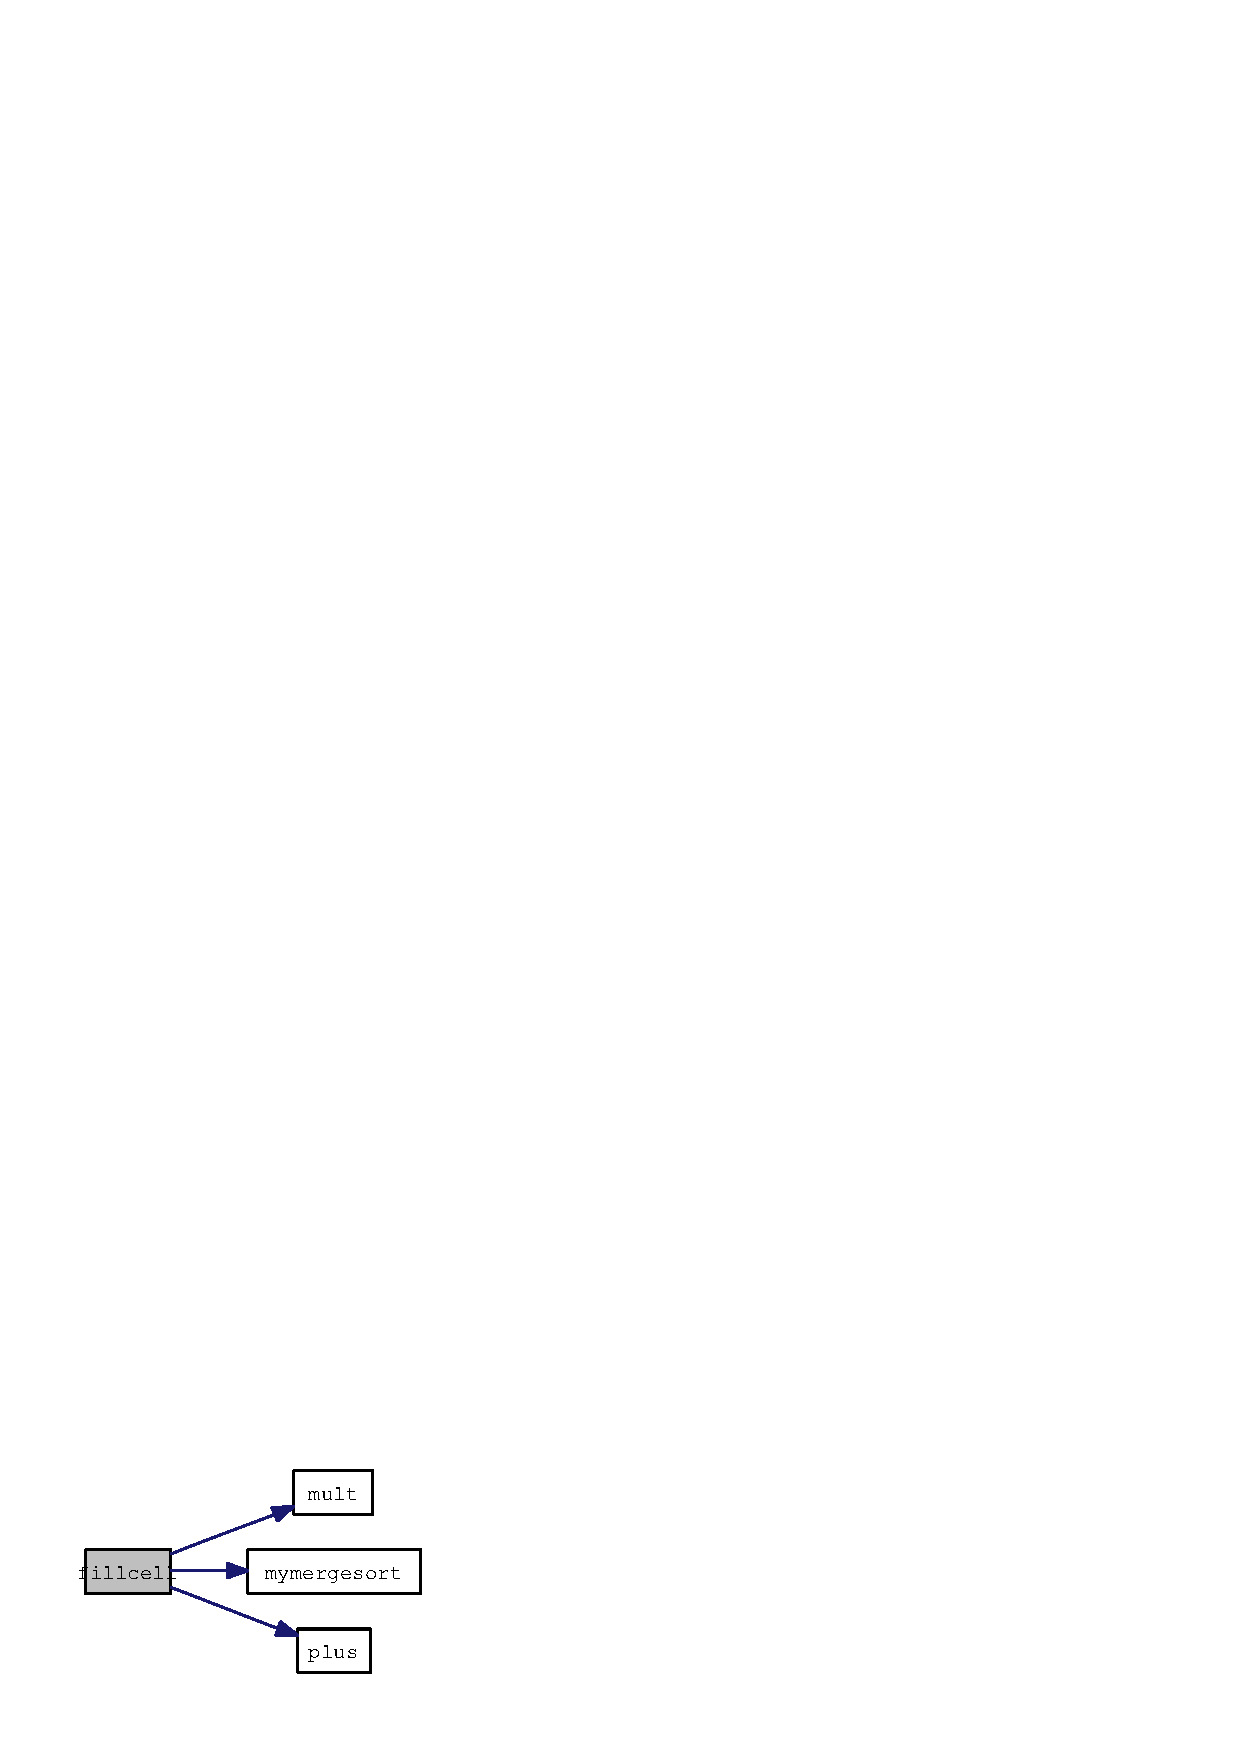
\includegraphics[width=98pt]{vandeWiel_8c_59f513c0ee260be89ad37daacf49e7e8_cgraph}
\end{center}
\end{figure}
\hypertarget{vandeWiel_8c_f72cc4501998ae01067d5555382b1609}{
\index{vandeWiel.c@{vandeWiel.c}!FreeW@{FreeW}}
\index{FreeW@{FreeW}!vandeWiel.c@{vandeWiel.c}}
\subsubsection[{FreeW}]{\setlength{\rightskip}{0pt plus 5cm}void FreeW (int {\em a}, \/  {\bf celW} $\ast$$\ast$ {\em W})}}
\label{vandeWiel_8c_f72cc4501998ae01067d5555382b1609}




Definition at line 81 of file vandeWiel.c.

Referenced by R\_\-split\_\-up\_\-2sample().\hypertarget{vandeWiel_8c_402c3e72a2fa3d600d4a4e8ace9f040b}{
\index{vandeWiel.c@{vandeWiel.c}!initW@{initW}}
\index{initW@{initW}!vandeWiel.c@{vandeWiel.c}}
\subsubsection[{initW}]{\setlength{\rightskip}{0pt plus 5cm}void initW (int {\em a}, \/  int {\em b}, \/  {\bf celW} $\ast$$\ast$ {\em W})}}
\label{vandeWiel_8c_402c3e72a2fa3d600d4a4e8ace9f040b}




Definition at line 91 of file vandeWiel.c.

References celW::c, celW::length, and celW::x.

Referenced by R\_\-split\_\-up\_\-2sample().\hypertarget{vandeWiel_8c_fb521caca26031c6fa9e92450685f5d1}{
\index{vandeWiel.c@{vandeWiel.c}!makeW@{makeW}}
\index{makeW@{makeW}!vandeWiel.c@{vandeWiel.c}}
\subsubsection[{makeW}]{\setlength{\rightskip}{0pt plus 5cm}void makeW ({\bf celW} $\ast$$\ast$ {\em W}, \/  int {\em a}, \/  int {\em b}, \/  int {\em start}, \/  double $\ast$ {\em rs})}}
\label{vandeWiel_8c_fb521caca26031c6fa9e92450685f5d1}




Definition at line 281 of file vandeWiel.c.

References fillcell(), and mirrorW().

Referenced by R\_\-split\_\-up\_\-2sample().

Here is the call graph for this function:\nopagebreak
\begin{figure}[H]
\begin{center}
\leavevmode
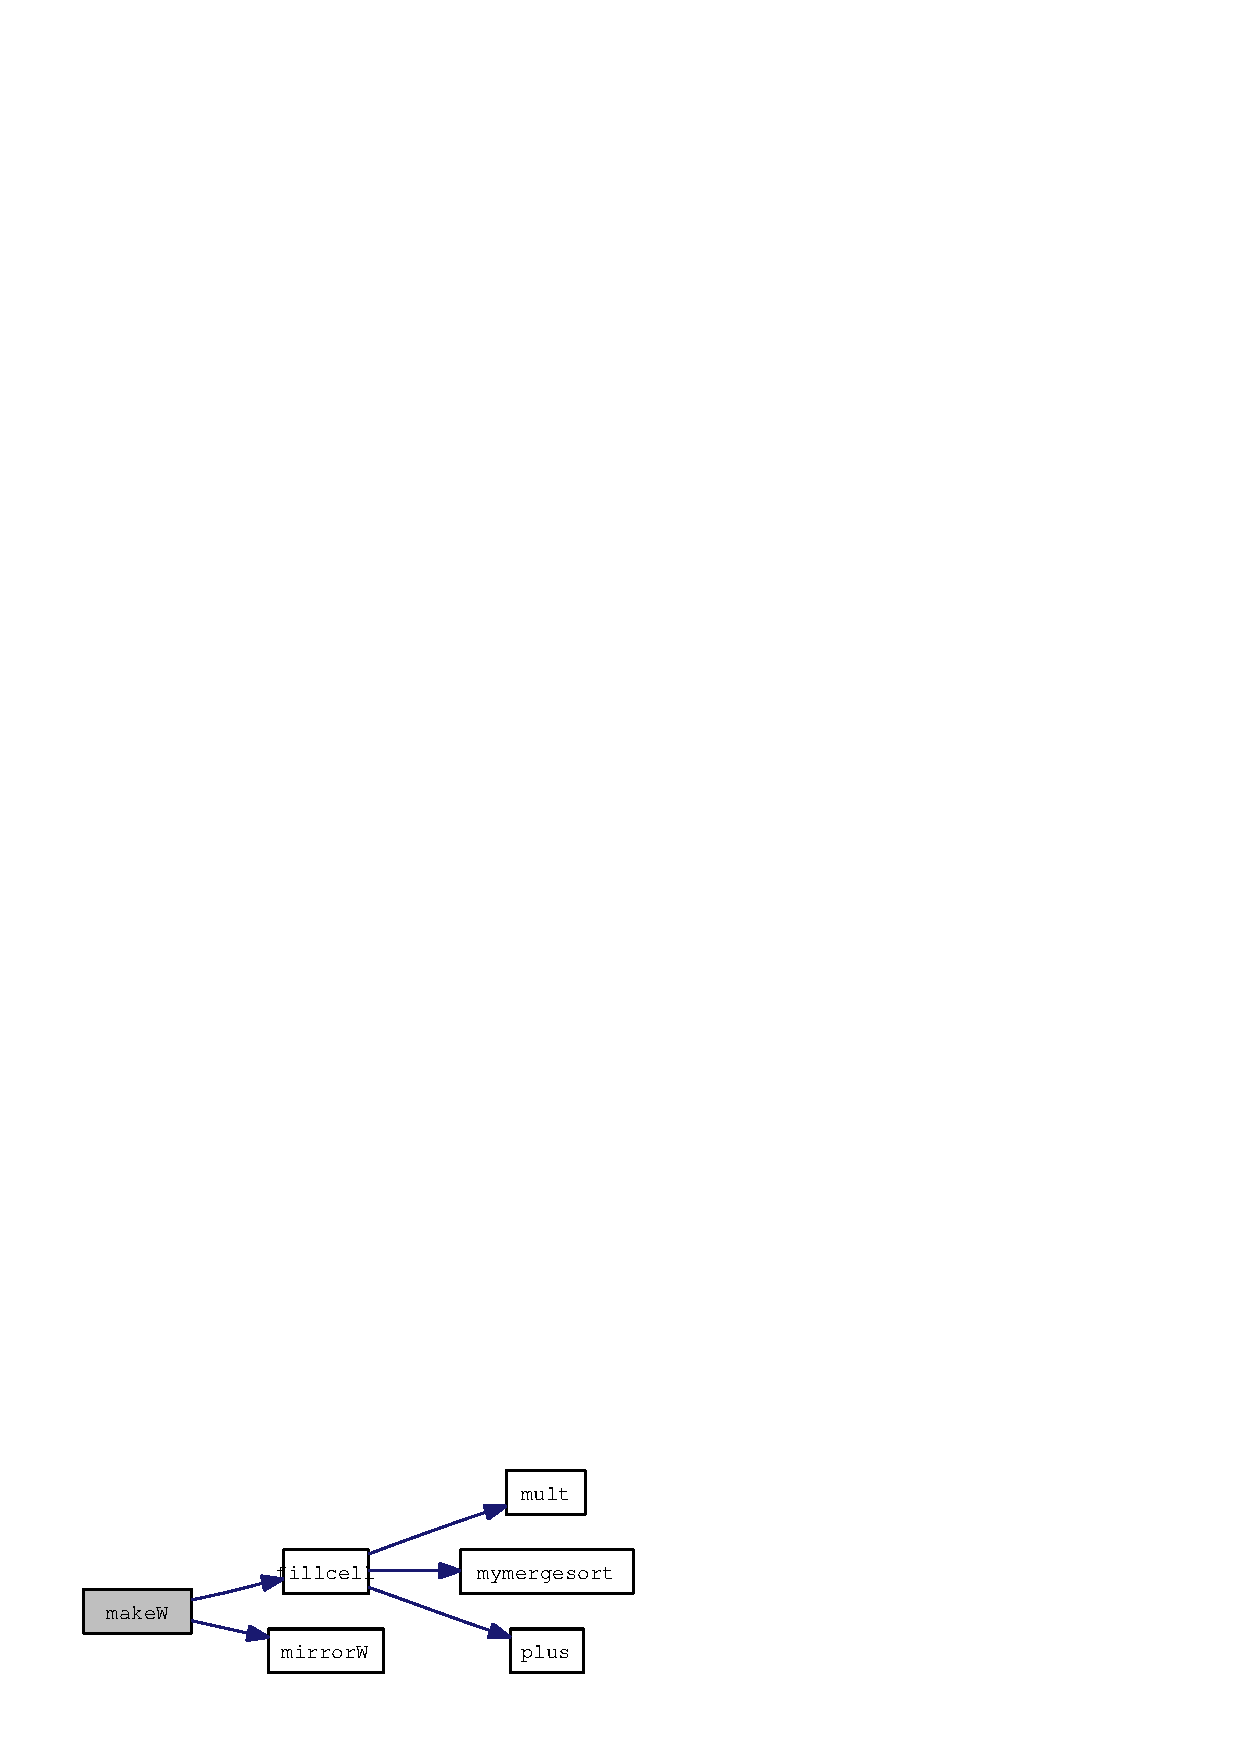
\includegraphics[width=145pt]{vandeWiel_8c_fb521caca26031c6fa9e92450685f5d1_cgraph}
\end{center}
\end{figure}
\hypertarget{vandeWiel_8c_d0195ffa22342dfadee0abeb564931dc}{
\index{vandeWiel.c@{vandeWiel.c}!mirrorW@{mirrorW}}
\index{mirrorW@{mirrorW}!vandeWiel.c@{vandeWiel.c}}
\subsubsection[{mirrorW}]{\setlength{\rightskip}{0pt plus 5cm}void mirrorW ({\bf celW} $\ast$$\ast$ {\em W}, \/  int {\em ce}, \/  int {\em bep}, \/  int {\em start}, \/  double $\ast$ {\em rs})}}
\label{vandeWiel_8c_d0195ffa22342dfadee0abeb564931dc}




Definition at line 257 of file vandeWiel.c.

References celW::c, celW::length, and celW::x.

Referenced by makeW().\hypertarget{vandeWiel_8c_e1d7e7e209f5b99745c8bca03057f761}{
\index{vandeWiel.c@{vandeWiel.c}!mult@{mult}}
\index{mult@{mult}!vandeWiel.c@{vandeWiel.c}}
\subsubsection[{mult}]{\setlength{\rightskip}{0pt plus 5cm}void mult ({\bf celW} $\ast$ {\em tem}, \/  int {\em a}, \/  int {\em b}, \/  int {\em rank}, \/  double $\ast$ {\em rs})}}
\label{vandeWiel_8c_e1d7e7e209f5b99745c8bca03057f761}




Definition at line 106 of file vandeWiel.c.

References celW::length.

Referenced by fillcell().\hypertarget{vandeWiel_8c_2f117e88849518e50d7d0eef3af07bf0}{
\index{vandeWiel.c@{vandeWiel.c}!mymergesort@{mymergesort}}
\index{mymergesort@{mymergesort}!vandeWiel.c@{vandeWiel.c}}
\subsubsection[{mymergesort}]{\setlength{\rightskip}{0pt plus 5cm}void mymergesort ({\bf celW} {\em temptw}, \/  long {\em tijd})}}
\label{vandeWiel_8c_2f117e88849518e50d7d0eef3af07bf0}




Definition at line 159 of file vandeWiel.c.

References celW::c, celW::length, and celW::x.

Referenced by fillcell().\hypertarget{vandeWiel_8c_14307006f6d9ec07bdfce7e853665bc5}{
\index{vandeWiel.c@{vandeWiel.c}!numbersmall@{numbersmall}}
\index{numbersmall@{numbersmall}!vandeWiel.c@{vandeWiel.c}}
\subsubsection[{numbersmall}]{\setlength{\rightskip}{0pt plus 5cm}double numbersmall (int {\em c}, \/  int {\em b}, \/  double {\em ob}, \/  {\bf celW} $\ast$$\ast$ {\em W1}, \/  {\bf celW} $\ast$$\ast$ {\em W2})}}
\label{vandeWiel_8c_14307006f6d9ec07bdfce7e853665bc5}




Definition at line 335 of file vandeWiel.c.

References celW::c, and celW::length.

Referenced by R\_\-split\_\-up\_\-2sample().\hypertarget{vandeWiel_8c_965c6db84dd8be42e1313d8c3ef9a784}{
\index{vandeWiel.c@{vandeWiel.c}!plus@{plus}}
\index{plus@{plus}!vandeWiel.c@{vandeWiel.c}}
\subsubsection[{plus}]{\setlength{\rightskip}{0pt plus 5cm}void plus ({\bf celW} $\ast$$\ast$ {\em W}, \/  {\bf celW} $\ast$ {\em tempie}, \/  int {\em a}, \/  int {\em b})}}
\label{vandeWiel_8c_965c6db84dd8be42e1313d8c3ef9a784}




Definition at line 120 of file vandeWiel.c.

References celW::c, celW::length, and celW::x.

Referenced by fillcell().\hypertarget{vandeWiel_8c_a50657b564a35ab41b3e3e50e62c51b1}{
\index{vandeWiel.c@{vandeWiel.c}!R\_\-split\_\-up\_\-2sample@{R\_\-split\_\-up\_\-2sample}}
\index{R\_\-split\_\-up\_\-2sample@{R\_\-split\_\-up\_\-2sample}!vandeWiel.c@{vandeWiel.c}}
\subsubsection[{R\_\-split\_\-up\_\-2sample}]{\setlength{\rightskip}{0pt plus 5cm}SEXP R\_\-split\_\-up\_\-2sample (SEXP {\em scores}, \/  SEXP {\em m}, \/  SEXP {\em obs})}}
\label{vandeWiel_8c_a50657b564a35ab41b3e3e50e62c51b1}




Definition at line 375 of file vandeWiel.c.

References binomi(), cumulcoef(), FreeW(), initW(), makeW(), numbersmall(), and reserveW().

Here is the call graph for this function:\nopagebreak
\begin{figure}[H]
\begin{center}
\leavevmode
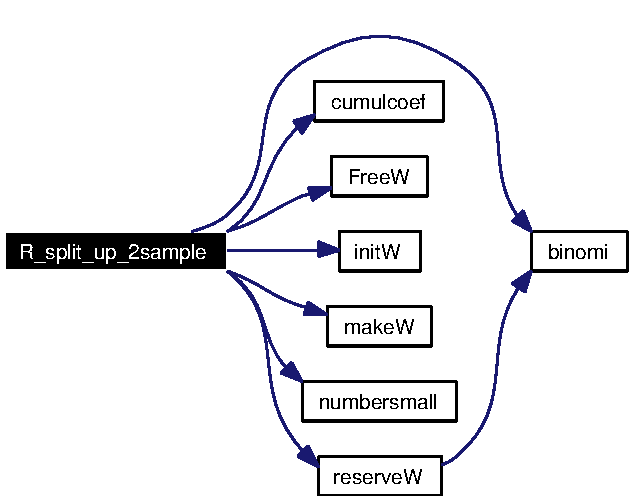
\includegraphics[width=226pt]{vandeWiel_8c_a50657b564a35ab41b3e3e50e62c51b1_cgraph}
\end{center}
\end{figure}
\hypertarget{vandeWiel_8c_03d7f636d17008a6fbe230458a92ddba}{
\index{vandeWiel.c@{vandeWiel.c}!reserveW@{reserveW}}
\index{reserveW@{reserveW}!vandeWiel.c@{vandeWiel.c}}
\subsubsection[{reserveW}]{\setlength{\rightskip}{0pt plus 5cm}{\bf celW}$\ast$$\ast$ reserveW (int {\em a}, \/  int {\em b})}}
\label{vandeWiel_8c_03d7f636d17008a6fbe230458a92ddba}




Definition at line 51 of file vandeWiel.c.

References binomi(), celW::c, and celW::x.

Referenced by R\_\-split\_\-up\_\-2sample().

Here is the call graph for this function:\nopagebreak
\begin{figure}[H]
\begin{center}
\leavevmode
\includegraphics[width=92pt]{vandeWiel_8c_03d7f636d17008a6fbe230458a92ddba_cgraph}
\end{center}
\end{figure}

\printindex
\end{document}
